% CODIGO DE ORDENACIONES
\definecolor{lightergray}{RGB}{247,247,247}
\definecolor{darkgreen}{RGB}{36,135,20}
\definecolor{green_comment}{RGB}{0,128,0}
\definecolor{redcell}{RGB}{238,176,176}
\definecolor{greencell}{RGB}{217,234,211}



\chapter{Estudio empírico}
\label{cap:c4_estudio}	
Después de diseñar e implementar las estrategias descritas en la Sección 3, llevamos a cabo un análisis exhaustivo para evaluar los tiempos de ejecución, realizar pruebas, contrastar resultados y extraer conclusiones

Primero, se ejecutan distintas pruebas en un ordenador de propósito general. Seguidamente ejecutar las mejores implementaciones en un sistema distribuido con un número elevado de núcleos de CPU. 

\section{Entornos de ejecución}

Para ejecutar las pruebas y comprobar el funcionamiento de las implementaciones, primero se ejecutan en un ordenador de propósito general. Este sistema computacional tiene las siguientes especificaciones:

\begin{itemize}
	\item Procesador (CPU): \textit{AMD Ryzen 7}, con 8 núcleos y 16 hilos, es capaz de defenderse con cargas de trabajo y paralelismo de alto nivel.
	\item Memoria (RAM): 32 GB de \textit{RAM DDR4}, permitiendo una amplia capacidad para manejar grandes volúmenes de datos en memoria. Característica fundamental para ejecutar algoritmos de IA que demandan una cantidad elevada de recursos.
	\item Tarjeta Gráfica (GPU): \textit{NVIDIA GeForce RTX 3070} con arquitectura \textit{Ampere} \cite{pool2020accelerating}, que cuenta con 5888 núcleos CUDA y 8 GB de memoria GDDR6. La arquitectura \textit{Ampere} es sucesora de la arquitectura \textit{Turing} lanzada en 2020. Fue diseñada para brindar un mejor rendimiento, especialmente en aplicaciones de computación paralela.
	\item Placa Base: \textit{X570 Gaming}. Soporta las tecnologías de conectividad de alta velocidad, garantizando el rendimiento y estabilidad del sistema en condiciones de carga elevada.
\end{itemize}

El sistema altamente distribuido, consta de tres ordenadores. Uno que funciona de Front-End y dos como nodos de cómputo, en total 128 núcleos y 256GB de RAM. La figura \ref{fig:cluster} muestra la estructura del cluster.




El Front-End, realiza la conexión remota con los otros dos ordenadores, situados en la Facultad de Informática de la Universidad Complutense de Madrid. Este ordenador no participa en el cómputo, solo mantiene los \textit{scripts} (tipo de fichero de texto con el código escrito en un lenguaje de programación, en este caso Python) y conecta los dos nodos de cómputo para que realicen las tareas.  Durante las pruebas, cada proceso tiene un núcleo dedicado, por lo que el rendimiento de cada proceso no se ve afectado por otros procesos del sistema. Esto permite mayor precisión para evaluar el rendimiento del sistema, y las pruebas ejecutadas no compiten por los recursos de la CPU. 


\vspace*{0.2cm}

\begin{figure}[!h]
	\centering
	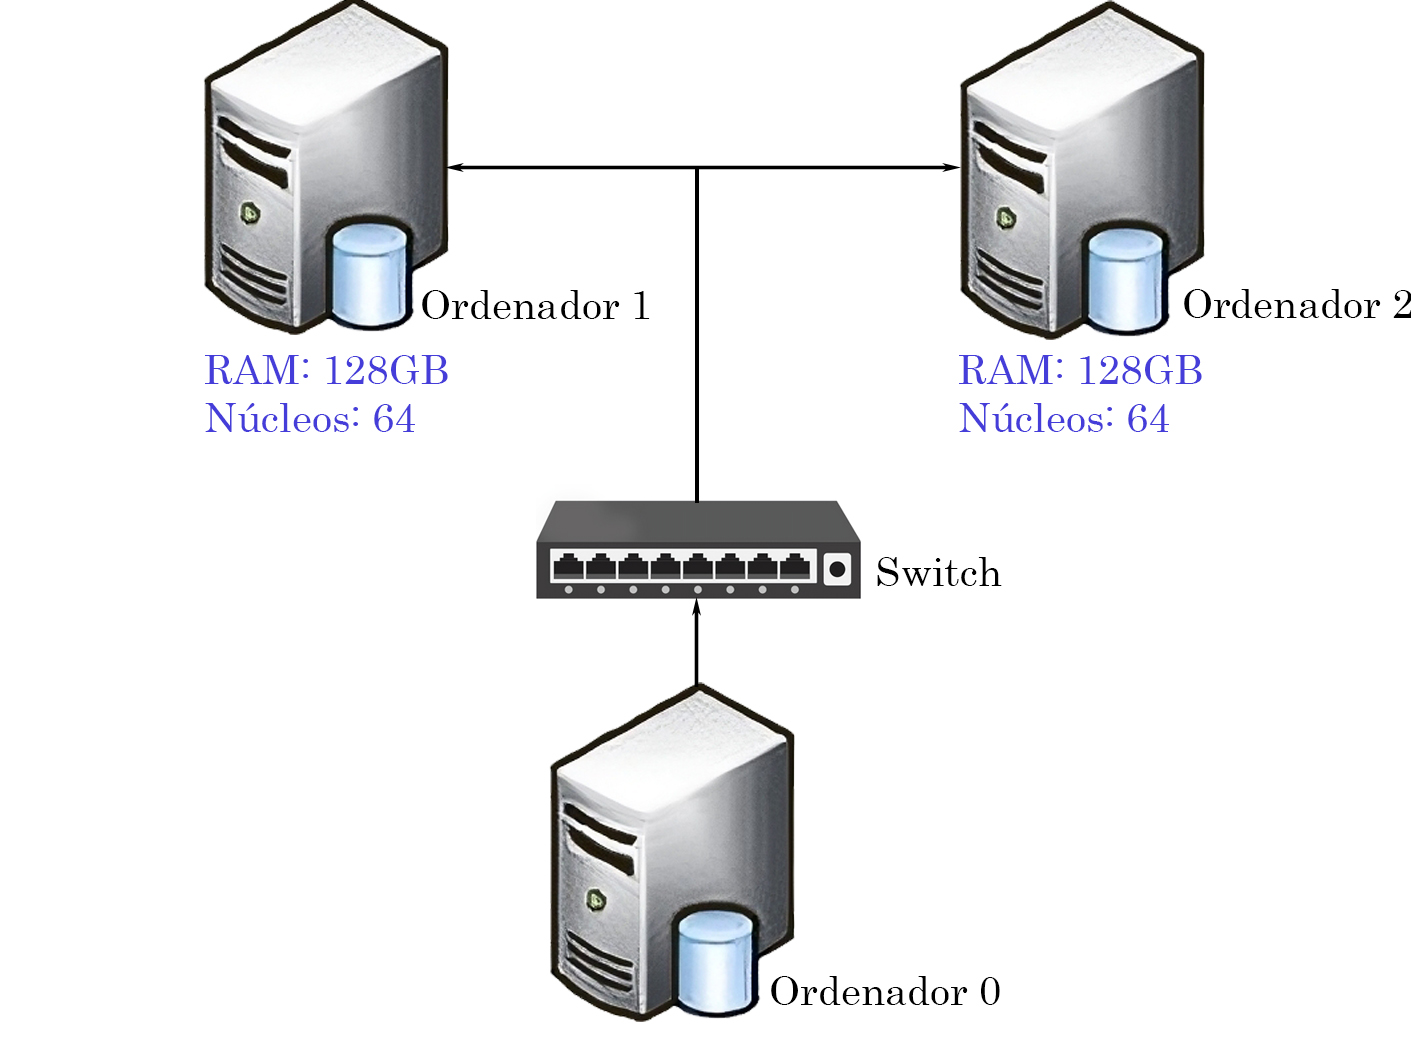
\includegraphics[width=0.5\textwidth]{images/chapter_4/cluster}
	\caption{MPI - Matriz}
	\label{fig:cluster}
\end{figure}

En un ordenador de propósito general esto no ocurre, pues están diseñados para ejecutar múltiples procesos simultáneamente, cada uno pudiendo requerir acceso a los mismos recursos del sistema, como la memoria RAM, disco duro o la CPU.

Para realizar las pruebas se usan las funciones \textit{open()} y \textit{write()} de Python para almacenar los tiempos de ejecución en ficheros de texto. Los tiempos se miden con las funciones de
tiempo de MPI, MPI.Wtime().

\section{Programas sencillos}

Primero realizamos el estudio de los programas básicos descritos en la Seccion \ref{cap:c3_1}, ordenación de arrays y multiplicación de matrices.

	% ------------------------------------------------------------------------------------------------
	% --- ORDENACIONES  ------------------------------------------------------------------------------
	% ------------------------------------------------------------------------------------------------
	\subsection{Ordenaciones}
	
	Las pruebas realizadas para estos algoritmos se realizan para el peor de los casos, es decir, un array de enteros sin repeticiones ordenado de forma decreciente. Cada algoritmo tiene que hacer el mayor número de comparaciones posibles para ordenar el array de manera creciente. El resultado de cada prueba (tiempo de ejecución en segundos) es almacenado en un fichero de texto y aumentado el tamaño del array para ejecutar la siguiente prueba, así hasta llegar a \textit{100.000} elementos.	
	
		\subsubsection{Algoritmos de complejidad cuadrática}		
		\label{cap:4_2_1_1}
		
		Debido al coste cuadrático de estos algoritmos, el incremento entre pruebas del tamaño de los arrays se obtiene de la siguiente forma:
		\begin{itemize}
			\vspace*{-0.2cm}	
			\item \([20-1.000)\) $\rightarrow$ 20 elementos.
			\vspace*{-0.4cm}	
			\item \([1.000-10.000)\) $\rightarrow$ 250 elementos.
			\vspace*{-0.4cm}	
			\item \([10.000-100.000)\) $\rightarrow$ 1.000 elementos.					
		\end{itemize}
		
		
		%\subsubsection{Algoritmo \textit{SequentialSort} aplicando las estrategias de HPC}			
		
		\textit{SelectionSort} es fácilmente paralelizable, pues para cada elemento se comprueba cuantos elementos en el array son mayores. Las estrategias implementadas utilizan el modelo \textit{Master-Worker}. El \textit{master} envía a cada proceso \textit{worker} un elemento del array para que hagan las comparaciones y devuelvan el indice del elemento, junto con el número de elementos mayores que el recibido, y así el \textit{master} se encarga de ordenar el array y enviar elementos sin procesar. La figura \ref{fig:sequentialsort_mpi} muestra los tiempos de ejecución. En rojo el algoritmo sin mejora, y en verde y negro la dos estrategias estrategias ejecutadas con cinco procesos. Se puede apreciar una considerable reducción del tiempo de ejecución. 
		
		Al comparar las dos estrategias MPI, se obtiene que la primera estrategia es un \textit{34\%} más rápida que la segunda. Sin embargo, la segunda estrategia tiene una menor complejidad espacial, mostrando en la gráfica de la derecha, en negro, que la memoria no varía al aumentar los procesos ejecutados.
						
		% Sequential sort + Uso de memoria
		\begin{figure}[h!]
			\centering
			\begin{tikzpicture}
				\begin{groupplot}[group style={
						group size=2 by 1,
						horizontal sep=1.5cm, 
						vertical sep=0.5cm}, 
					grid=major,
					width=0.5\textwidth, height=0.37\textwidth, 
					tick label style={font=\tiny}
					]
					
					% Grafico de la izquierda --------------
					\nextgroupplot[
					title={}, 
					ylabel=Tiempo (s), 
					xlabel=Tam. Array ($10^4$),
					legend pos=north west,					
					scaled x ticks=false,
					]
					\addplot [mark=none, color=red, line width=1.2pt] table [x index=0, y index=1, col sep=space] {files/sequential.txt};
					\addplot [mark=none, color=darkgreen, line width=1.2pt] table [x index=0, y index=2, col sep=space] {files/sequential.txt};
					\addplot [mark=none, color=black, line width=1.2pt] table [x index=0, y index=3, col sep=space] {files/sequential.txt};
					
					% Leyendas
					\addlegendentry{Básico}
					\addlegendentry{MPI\_1}
					\addlegendentry{MPI\_2}
					
					% Grafico de la derecha --------------
					\nextgroupplot[
					title={},
					xtick={2,3,4,5,6,7,8,9,10}, 
					ytick={0,2,4,6,8,10,12}, 
					legend pos=north west,			
					xlabel=Num. Procesadores,
					ylabel=Memoria \tiny(Copias del array)
					]
					\addplot[name path=darkgreen, color=darkgreen, mark=square] table {files/sequentialMem.txt};
					
					
					\addplot[name path=black, color=black, mark=triangle] table [y index=2] {files/sequentialMem.txt};
					
					
					\addplot [color=darkgreen!50, fill=darkgreen!50, fill opacity=0.3] fill between [of=darkgreen and black, soft clip={domain=2:10}];
					
					\addplot [name path=axis, draw=none] coordinates {(2,0) (10,0) };	
					
					\addplot [color=black!50, fill=black!50, fill opacity=0.3] fill between [of=black and axis, soft clip={domain=2:10}];
					
					% Leyendas
					\addlegendentry{MPI\_1}
					\addlegendentry{MPI\_2}
					
				\end{groupplot}  				
			\end{tikzpicture}
			\caption{SequentialSort - Tiempos de ejecución de las estrategias MPI y su uso de Memoria}
			\label{fig:sequentialsort_mpi}
		\end{figure}
		
	
		
		%Primero ejecutamos las pruebas para los algoritmos sin mejora, comprobando así cual es el mejor.
		
		Una vez comparado las estrategias MPI con el algoritmo secuencial, podemos comprobar el rendimiento frente a los algoritmos famosos. La figura \ref{fig:ordenaciones_cuadraticas} muestra que \textit{SelectionSort} (la función de color negro) es la ordenación que mejores resultados obtiene, y \textit{BubbleSort} (la roja) la que peores. \textit{SelectionSort} es, aproximadamente, \textit{3.5} veces más rápida al ordenar \textit{70.000} elementos. La ordenación \textit{SequentialSort} sin paralelizar, es incluso más rápida que dos de las más famosas. Esto es debido a la simpleza de las operaciones aplicadas en la ordenación, pues solo hace \(N^{2}\) comparaciones. En \textit{BubbleSort} e \textit{InsertionSort}, además de realizar comparaciones, modifican las posiciones de los elementos en el array, aumentando el tiempo de ejecución.
		
		La estrategia MPI de \textit{SequentialSort} que menos tiempo consume (la primera) no obtiene mejores resultados que la mejor ordenación sin mejoras (\textit{SelectionSort}) hasta llegar a los cuatro procesadores ejecutados, siendo un \textit{20\%} más veloz. Para mostrar de forma más clara la diferencia de tiempos entre estas dos ordenaciones, se muestra la ejecución de la primera estrategia con cinco procesadores, obteniendo un \textit{50\%} de mejora.
		
		
		\begin{figure}[!h]
			\centering
			\begin{tikzpicture}
			\begin{axis}[
				xlabel={Tam. Array ($10^4$)},
				ylabel={Tiempo (s)},
				xtick={0,1,2,3,4,5,6,7,8},
				legend pos=north west,
				grid=major,
				width=0.70\textwidth,
				height=0.4\textwidth,
				scaled x ticks=false,
				]				
				
				\addplot [mark=none, color=red, line width=1.2pt] table [x index=0, y index=1, col sep=space] {files/sortn2.txt};
				\addplot [mark=none, color=blue, line width=1.2pt] table [x index=0, y index=2, col sep=space] {files/sortn2.txt};
				\addplot [mark=none, color=black, line width=1.2pt] table [x index=0, y index=3, col sep=space] {files/sortn2.txt};
				\addplot [mark=none, color=magenta, line width=1.2pt] table [x index=0, y index=4, col sep=space] {files/sortn2.txt};
				\addplot [mark=none, color=darkgreen, line width=1.2pt] table [x index=0, y index=5, col sep=space] {files/sortn2.txt};
				
			
				\addlegendentry{Bubble}
				\addlegendentry{Insertion}
				\addlegendentry{Selection}
				\addlegendentry{Sequential}
				\addlegendentry{Sequential\_MPI(5)}
					
			\end{axis}
			\end{tikzpicture}
			\caption{Tiempo de ejecución de los algoritmos de ordenación cuadráticos}
			\label{fig:ordenaciones_cuadraticas}
		\end{figure}
		
		
		\subsubsection{Algoritmo \textit{MergeSort}}
		
		Este algoritmo no tiene un coste tan elevado como los anteriores. La complejidad es logarítmica O(NLogN) lo que provoca que se pueda aumentar el tamaño del array a ordenar. Para la estrategia implementada, no se aplica el modelo \textit{Master-Worker}, todos los procesos creados trabajan de manera igualitaria. Como se dijo en la seccion \ref{cap:c3_1}, esta estrategia usa potencias de dos procesos para ordenar el array. En cada iteración los procesos se comunican con el más cercano, uno le envía su subarray ordenado y termina su ejecución (el de mayor \textit{id} de cada pareja), mientras que el otro reordena los dos subarrays y continua a la siguiente iteración.
					
		
		En esta ocasión, la prueba realizada consiste en ordenar de manera creciente cuatro arrays de enteros inicializados de manera decreciente (peor de los casos), empezando con \textit{25.000} elementos e incrementar esa misma cantidad entre pruebas. Pese a tener solo ocho núcleos en el ordenador de propósito general, se comprueba el rendimiento de la estrategia con \textit{4}, \textit{8}, \textit{16} y \textit{32} procesos. La figura \ref{fig:mergesort_hist} muestra los resultados obtenidos en forma de histograma. Como la estrategia aplica ordenaciones cuadráticas en los subarrays al comienzo del algoritmo, no se obtienen buenos resultados con pocos procesos, debido al elevado tamaño del array a ordenar. Con dos procesos ejecutándose no reduce el tiempo de ejecución, lo duplica. El cómputo es equivalente a aplicar una ordenación cuadrática con la mitad del array a ordenar. No obstante, se puede apreciar una notoria reducción del tiempo de ejecución apartir de \textit{16} procesos, llegando a tener un speedup aproximado de \textit{15.5}. Es cierto que se podrían aplicar otras ordenaciones con menor complejidad para reducir más el tiempo, pero así se demuestra que en la computación de alto rendimiento se pueden obtener buenos resultados con estrategias no tan efectivas pero bien paralelizadas.
		
		% HISTOGRAMA CON VARIOS PROCESOS
		\begin{figure}[!h]
		\begin{tikzpicture}
			\begin{axis}[
				ybar,
				bar width=0.35cm,
				ylabel={Tiempo de ejecución (s)},
				xlabel={Tam. array ($10^3$)},
				symbolic x coords={25, 50, 75, 100},
				xtick=data,
				enlarge x limits=0.2,
				ymin=0,
				%width=15cm,
				%height=10cm,
				width=\textwidth,
				height=0.38\textwidth,
				legend style={at={(0.5,1.16)}, anchor=north, legend columns=-1},
				area legend
				]
				
				\addplot+[ybar, pattern=vertical lines, draw=black] plot coordinates 
				{(25, 1.12) (50, 4.39) (75, 10.0) (100, 21)};
				\addplot+[ybar, pattern=grid, draw=black] plot coordinates 
				{(25, 0.67) (50, 2.58) (75, 5.70) (100, 10.15) };
				\addplot+[ybar, pattern=dots, draw=black] plot coordinates 
				{(25, 0.23) (50, 0.93) (75, 2.09) (100, 3.35) };
				\addplot+[ybar, pattern=crosshatch, draw=black] plot coordinates 
				{(25, 0.09) (50, 0.34) (75, 0.72) (100, 1.39)};
				\addplot+[ybar, pattern=checkerboard, draw=black] plot coordinates 
				{(25, 0.059) (50, 0.18) (75, 0.41) (100, 0.71)};
				
				
				\legend{Secuencial, MPI(4),MPI(8),MPI(16),MPI(32)}
			\end{axis}	
		\end{tikzpicture}
		\caption{Tiempo de ejecución del algoritmo \textit{MergeSort} en ordenador de propósito general}
		\label{fig:mergesort_hist}
		\end{figure}
		
			
		
		La memoria está optimizada, puesto que el array esta dividido entre los procesos. Al terminar un proceso con la sincronización en mariposa comentada en la sección \ref{cap:c3_1}, se termina la ejecución del proceso liberando memoria una vez ha enviado al proceso correspondiente su subarray ordenado.
		
		\newpage
		
		
		%%\subsubsection{Cluster}
		Habiendo obtenido buenos resultados con muchos procesos, pasamos a comentar las pruebas realizadas en el sistema altamente distribuido.
		
		El algoritmo secuencial de \textit{MergeSort} tarda unos \textit{20.16} segundos en ordenar de manera creciente, un array de \textit{100.000} elementos ordenados de manera decreciente (el peor de los casos). Por esos se realiza una prueba para saber cuanto tiempo tarda la estrategia en ordenar un array con un millón de elementos. Las pruebas comienzan con \textit{100.000} elementos, incrementando nueve veces su tamaño hasta llegar al millón de elementos. Estas pruebas se realizan con \textit{16}, \textit{32}, \textit{64} y \textit{128} procesos. La figura \ref{fig:mergesort_cluster} muestra los resultados obtenidos. 
		
		De manera secuencial, sin mejoras, el algoritmo tarda, \textit{20.16} segundos en ordenar \textit{100.000} elementos, mientras que con 128 procesos tarda \textit{0.16} segundos, obteniendo un \textit{speedup} de \textit{125}. 
		
		\begin{figure}[!h]
			\centering
			\begin{tikzpicture}
			\begin{axis}[
				xlabel={Tam. Array ($10^5$)},
				ylabel={Tiempo de ejecución (s)},
				legend style={at={(1.02,0.5)}, anchor=west},
				grid=major,
				width=\textwidth,
				height=0.45\textwidth,				
				scaled x ticks=false,
				legend cell align={left},
				extra description/.code={
					\node at (1.01, 0.72) [anchor=west] {\textbf{Cores}};
				}
				]
				
				\addplot [mark=*, color=red, line width=1.2pt] table [x index=0, y index=1, col sep=space] {files/cluster/sort.txt};
				\addplot [mark=square*, color=blue, line width=1.2pt] table [x index=0, y index=2, col sep=space] {files/cluster/sort.txt};
				\addplot [mark=triangle*, color=black, line width=1.2pt] table [x index=0, y index=3, col sep=space] {files/cluster/sort.txt};
				\addplot [mark=star, color=darkgreen, line width=1.2pt] table [x index=0, y index=4, col sep=space] {files/cluster/sort.txt};
				
				
				\addlegendentry{16}
				\addlegendentry{32}
				\addlegendentry{64}
				\addlegendentry{128}
				
				
			\end{axis}
			\end{tikzpicture}
			\caption{Tiempo de ejecución del algoritmo \textit{MergeSort} en Cluster}
			\label{fig:mergesort_cluster}
		\end{figure}
		
		Al incrementar del tamaño del array, todas las pruebas funcionan correctamente. Ejecutar el algoritmo secuencial con un millón de elementos tardaría mucho. Sin embargo, se puede hacer una estimación como muestra la tabla \ref{tab:estimacion_mergesort}, en la cual, aplicando factores de conversión, se obtiene que \textit{X = 241.67} segundos, y llegando a tener un \textit{speedup} de \textit{78} al aplicar \textit{128} procesos.
		
		\begin{table}[!h]
			\centering
			\begin{tabular}{|c|c|c|}
				\hline
				\rowcolor{lightgray}
				\textbf{Tamaño (N)} & \textbf{Funcion = N*Log2(N)} & \textbf{Tiempo (s)} \\
				\hline
				100000 & 1.66e06 & 20.16s \\
				\hline
				1000000 & 1.99e07 & X \\
				\hline
				
			\end{tabular}
			\caption{Estimación del tiempo de ejecución de \textit{MergeSort} con un millón de elementos}
			\label{tab:estimacion_mergesort}
		\end{table}
		
		

	% ------------------------------------------------------------------------------------------------
	% --- MATRIZ -------------------------------------------------------------------------------------
	% ------------------------------------------------------------------------------------------------
	\subsection{Multiplicación de matrices}
		
		Para este algoritmo, al contrario que los anteriores, no hay caso peor, pues siempre se ejecutan el mismo numero de multiplicaciones para cualquier combinación de una matriz. 
		
		Las pruebas se realizan con una única matriz cuadrada de tamaño \textit{2000}. Se genera de manera aleatoria con valores que oscilan entre \textit{[1-9]}, y es almacenada para usar en cada prueba. Inicialmente, la matriz empieza con diez filas y columnas, al finalizar una prueba, se almacena el tiempo de ejecución y se incrementa el tamaño en diez, así hasta llegar a \textit{1750} filas y columnas. 
		
		La distribución de tareas de los procesos se realiza mediante el modelo \textit{Master-Worker}. El proceso \textit{master} se encarga de enviar una matriz completa \textit{(B)}, y enviar filas de la matriz \textit{(A)} a los \textit{workers} para que realicen el cálculo de dicha fila. Al finalizar el procesado envían de vuelta la fila al \textit{master} y esperan otra fila sin procesar, para poder, al final de la ejecución formar, entre todos, la matriz final \textit{(C)}. \textit{(A*B=C)}
	
		Cada proceso necesita, al menos, una copia de una matriz completa. El uso de memoria es proporcional al número de procesos ejecutados. No hace falta tener las dos matrices porque el \textit{master} se encarga de repartir filas para que vayan realizando el cálculo.
		
		\vspace*{0.2cm}
	
		Seguidamente se ejecutan los programas de multiplicación de matrices en el ordenador de propósito general. La figura \ref{fig:mult_matrices} muestra la ejecución del algoritmo secuencial, además de la estrategia implementada en la sección \ref{cap:c3_1}, con \textit{2}, \textit{4} y \textit{6} procesos \textit{workers}. Se puede apreciar, la reducción, aplicando la estrategia con los diferentes números de procesos, llegando a obtener un \textit{speedup} de \textit{8.4} al ejecutar el algoritmo con seis \textit{workers} en una multiplicación de \textit{1750x1750}.
		
		\begin{figure}[!h]
		\centering
		\begin{tikzpicture}
			\begin{axis}[
				xlabel={Matriz (NxN)},
				ylabel={Tiempo de ejeución (s)},
				legend pos=north west,
				grid=major,
				width=\textwidth,
				height=0.4\textwidth
				]				

				\addplot [mark=none, color=red, line width=1.2pt] table [x index=0, y index=1, col sep=space] {files/multiplicacion1.txt};
				\addplot [mark=none, color=blue, line width=1.2pt] table [x index=0, y index=2, col sep=space] {files/multiplicacion1.txt};
				\addplot [mark=none, color=black, line width=1.2pt] table [x index=0, y index=3, col sep=space] {files/multiplicacion1.txt};
				\addplot [mark=none, color=darkgreen, line width=1.2pt] table [x index=0, y index=4, col sep=space] {files/multiplicacion1.txt};
							

				\addlegendentry{Secuencial}
				\addlegendentry{MPI(2)}
				\addlegendentry{MPI(4)}
				\addlegendentry{MPI(6)}
				
				
			\end{axis}
		\end{tikzpicture} 
		\caption{Tiempo de ejecución de multiplicación de matrices en ordenador de propósito general}
		\label{fig:mult_matrices}
		\end{figure}
		
		
		
		\newpage
		
		Las oscilaciones en la gráfica se deben al incremento de diez elementos entre pruebas en un algoritmo con complejidad cúbica O($N^{3}$). Estas oscilaciones son mas pronunciadas en la multiplicación sin paralelizar, pues el tiempo de ejecución es mayor.
		
		En el cluster, al poder ejecutar muchos procesos, se puede aumentar el tamaño de las matrices de las pruebas a ejecutar. Utilizamos \textit{16}, \textit{32}, \textit{64} y \textit{128} procesos para medir el tiempo que tarda el algoritmo con la misma estrategia que la prueba anterior. En este caso comenzando con \textit{500} elementos por fila, e incrementando ese mismo tamaño hasta llegar a una matriz de \textit{5000} filas y columnas. 
				
		La figura \ref{fig:mult_matrices_cluster} muestra los tiempos de ejecución con los procesos y tamaños comentados en el párrafo anterior. No se puede apreciar, pero con una matriz de \textit{1000} filas, ejecutar \textit{128} procesos reduce el tiempo de ejecución hasta unos \textit{1.06} segundos, logrando un \textit{speedup} de \textit{84} con respecto a los \textit{89.1} segundos del cálculo sin paralelizar. La comunicación entre procesos no es tan óptima como en la estrategia de \textit{MergeSort}, debido a que en esta implementación aplicamos el modelo \textit{Master-Worker} y es posible que un proceso \textit{worker}, al finalizar de procesar una fila, tenga que esperar a que el \textit{master} esté libre (puede estar recibiendo y colocando otros datos recibidos de otro proceso) para recibir nuevos datos que procesar. En cada prueba, se pierden \textit{(N/M)*T} segundos en la comunicación entre procesos. Siendo \textit{N} el número de filas de la matriz, \textit{M} el número de \textit{workers} y \textit{T} el tiempo de comunicación.

		\begin{figure}[!h]
			%\centering % AL QUITAR ESTA OPCION SE PUEDE MOVER LA FIGURA
			\hspace{-0.07\textwidth} 
			\begin{tikzpicture}
				\begin{axis}[
					xlabel={Tam. Matriz (NxN)},
					ylabel={Tiempo de ejecución (s)},
					legend style={at={(1.02,0.5)}, anchor=west},
					grid=major,
					width=\textwidth, 
					height=0.45\textwidth,
					legend cell align={left},
					extra description/.code={
						\node at (1.01, 0.72) [anchor=west] {\textbf{Cores}};
					}
					]
					
					\addplot [mark=*, color=red, line width=1.2pt] table [x index=0, y index=1, col sep=space] {files/cluster/mult.txt};
					\addplot [mark=square*, color=blue, line width=1.2pt] table [x index=0, y index=2, col sep=space] {files/cluster/mult.txt};
					\addplot [mark=triangle*, color=black, line width=1.2pt] table [x index=0, y index=3, col sep=space] {files/cluster/mult.txt};
					\addplot [mark=star, color=darkgreen, line width=1.2pt] table [x index=0, y index=4, col sep=space] {files/cluster/mult.txt};
					
					\addlegendentry{16}
					\addlegendentry{32}
					\addlegendentry{64}
					\addlegendentry{128}
					
				\end{axis}
			\end{tikzpicture}
			\caption{Tiempo de ejecución de multiplicación de matrices en Cluster}
			\label{fig:mult_matrices_cluster}
		\end{figure}
		
		
			
			
	
% ------------------------------------------------------------------------------------------------
% --- JERARQUICO AGLOMERATIVO --------------------------------------------------------------------
% ------------------------------------------------------------------------------------------------


\section{Algoritmos de Agrupación}

	Las poblaciones que se utilizan en las pruebas de esta sección se han almacenado en un fichero para usar la misma población generada de manera aleatoria, delimitando un intervalo \textit{[-10, 10]} para todas las dimensiones disponibles. Los tamaños de las poblaciones se incrementan dependiendo de la complejidad temporal de cada algoritmo. En sus secciones se especifica en profundidad.	
	
	Los tres algoritmos de esta sección, se basan en el modelos \textit{Master-Worker}. El \textit{master} divide los datos de entrada para que los \textit{workers} hagan el procesado. El \textit{master} en cada algoritmo tiene las siguientes funciones:	
	
	\begin{itemize}
		\item Jerarquico Aglomerativo. En cada iteración se encarga de gestionar que procesos tienen que eliminar o actualizar las filas y columnas de la matriz. El \textit{master} no tiene una copia de la matriz, así mejorando el uso de memoria al estar dividida entre los procesos \textit{workers}.
		\item KMedias. Su funcion principal es comprobar la condición de finalización. En cada iteración recibe las asignaciones de los datos procesados de los \textit{workers}, y si esta asignación no varía se finaliza la ejecución.
		\item K-Vecinos más Cercanos (KNN). En las dos estrategias se encarga, de diferente forma, de actualizar las poblaciones de los \textit{workers} para que haya mas precisión a la hora de categorizar nuevos individuos.
	\end{itemize} 

	%Los algoritmos de aprendizaje no supervisado, Jerárquico Aglomerativo y K-Medias, categorizan una población entera, y además tienen una complejidad cuadrática O(\(N^{2}\)). Por eso, para las pruebas, se incrementan las poblaciones de la siguiente forma:
	
	%\begin{itemize}
	%	\vspace*{-0.2cm}	
	%	\item \([20-1.000)\) $\rightarrow$ 20 elementos.
	%	\vspace*{-0.4cm}	
	%	\item \([1.000-10.000)\) $\rightarrow$ 250 elementos.
	%	\vspace*{-0.4cm}	
	%	\item \([10.000-100.000)\) $\rightarrow$ 1.000 elementos.					
	%\end{itemize}


	\subsection{Jerárquico Aglomerativo}
	
		De los tres algoritmos de agrupación, este es el más lento. Su bucle principal itera \textit{N-C} veces, siendo \textit{N} el numero de individuos de la población y \textit{C} el número de clusters deseados. En cada iteración, recorre una matriz entera para juntar dos clusters, los que se encuentren a menor distancia. 
		
	%\subsubsection{Distancias sin mejoras}		
		
		En este algoritmo, el cálculo de las distancias entre clusters es muy importante. Cada tipo genera diferentes agrupaciones, además de tener diferentes complejidades temporales. La distancia por \textit{centroides} es la que menos tiempo consume, siendo constante, al solo importar los centros de los clusters. Mientras que \textit{enlace simple} y \textit{completo} tienen una complejidad cuadrática O(\(N^{2}\)), recorriendo todos los individuos de los ambos clusters para calcular la distancia. Además hay que añadir el cálculo de la distancia entre individuos, que puede ser \textit{Manhattan} o Euclídea, siendo esta última un poco más tardía que la primera.
		

		Para mostrar la importancia de las distancias entre clusters y entre individuos, se realiza un estudio de los algoritmos sin aplicar ninguna estrategia computo de alto rendimiento (HPC). Con la población almacenada, se ejecutan las diferentes combinaciones de distancias (entre cluster e individuo), generando 4 tipos, pues enlace \textit{simple} y \textit{completo} solo varia almacenar la menor o menor distancia entre clusters. Empezando con veinte individuos, y aumentando ese mismo tamaño hasta llegar a mil. A partir de este punto, es mejor incrementar entre prueba \textit{250} individuos, pues ya empieza a tardar bastante. La figura \ref{fig:prueba_jerarquicosec} muestra dicho estudio. 
		
		Al principio no hay tanta diferencia, pero conforme aumenta el tamaño de la población, los tiempos de ejecución empiezan a distinguirse. Como muestra el circulo rojo, la distancia entre clusters por \textit{centroide} no varia mucho usar una distancia \textit{euclídea} o \textit{manhattan} entre individuos. No obstante, aplicando enlace \textit{simple} (o \textit{completo}) es mejor usar distancia \textit{manhattan}. El cálculo de distancias entre individuos no usa potencias o raices cuadradas, operaciones con un mayor coste que restas en valor absoluto. Cabe recalcar la diferencia de las distancias entre clusters por \textit{centroide} y por enlace \textit{simple} y \textit{completo}. Al aumentar la población a categorizar aumentan los tamaños de los clusters, sobrecargando el calculo de nuevas distancias.
		
		
		\begin{figure}[!h]
			\centering
			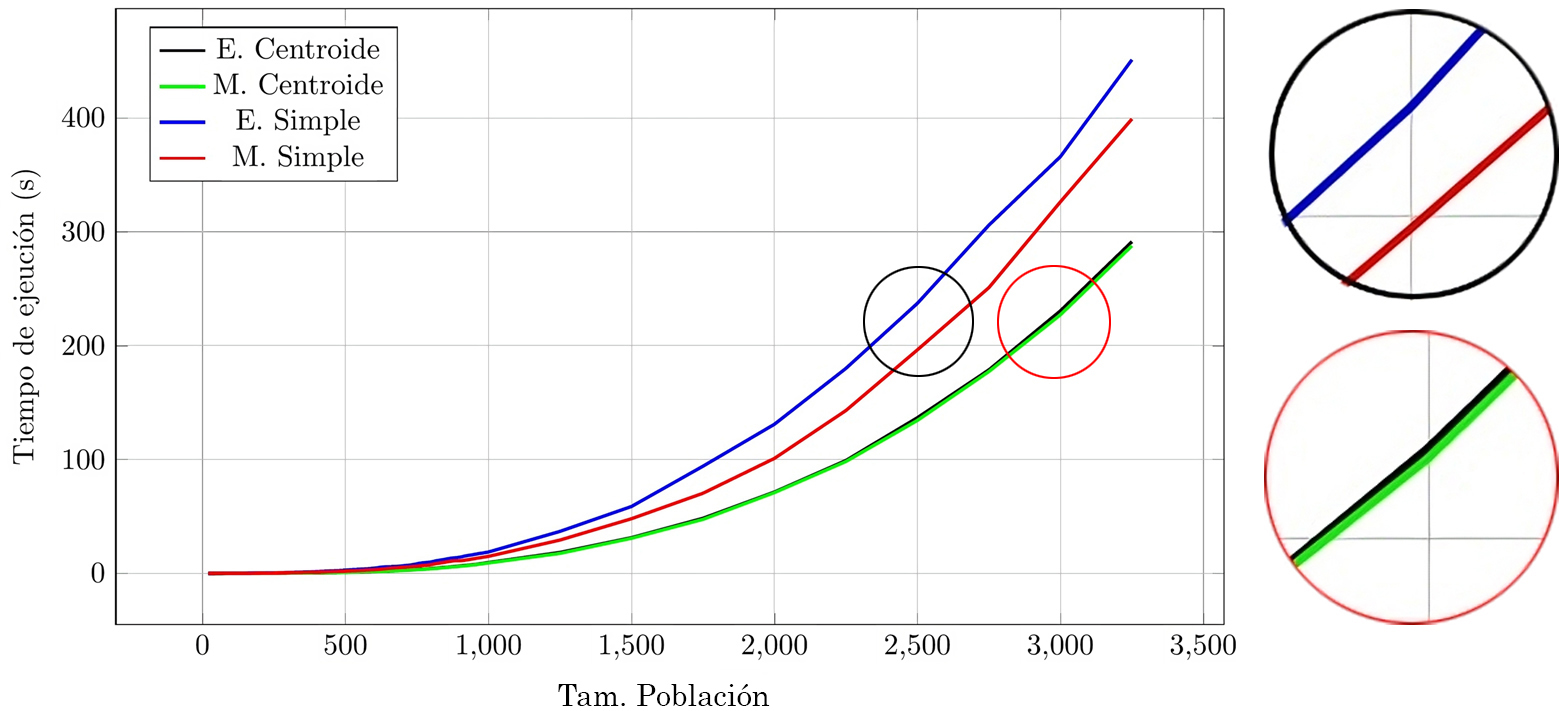
\includegraphics[width=0.8\textwidth]{images/chapter_4/jerarquico}
			\caption{Tiempo de ejecución de las combinaciones de distancias en el algoritmo secuencial Jerarquíco Aglomerativo}
			\label{fig:prueba_jerarquicosec}
		\end{figure}
	
			
			
		
		
	%\subsubsection{Distancia Centroide con mejoras}	
		Una vez comprobado los tiempos de ejecución del algoritmo sin paralelizar, podemos pasar a las pruebas de las estrategias comentadas en la sección \ref{cap:3_2_1}. Primero estudiamos la distancia entre cluster con menor tiempo de ejecución, por \textit{centroide}. Ejecutamos, con \textit{2}, \textit{4}, \textit{6} y \textit{8} procesos la primera estrategia en tres diferentes poblaciones. No aplicamos la segunda y tercera estrategia, pues estas están diseñadas para las distancias por enlace \textit{simple} y \textit{completo}.
		
		
		La figura \ref{fig:JA_centroide} muestra un buen rendimiento, reduciendo los tiempos de ejecución hasta con tamaños de poblaciones elevados. Para una población de \textit{5000} individuos se consiguen los siguientes \textit{speedups [1.78, 2.89, 3.61, 4.21]}. Los \textit{speedups} no crecen en proporción a los procesos ejecutados. La estrategia implementada, para tamaños de poblaciones elevados, no es optima. Si un proceso no elimina filas en muchas iteraciones, acumula muchos más datos que procesar que los demás procesos, provocando que los procesos con menos datos esperen para seguir con la ejecución.
			
		% JERARQUICO AGLOMERATIVO: HISTOGRAMA CON VARIOS PROCESOS
		\begin{figure}[!h]
		\centering
		\begin{tikzpicture}
		\begin{axis}[
			ybar,
			bar width=0.35cm,
			ylabel={Tiempo de ejecución (s)},
			xlabel={Tam. Array},
			symbolic x coords={1000, 2500, 5000},
			xtick=data,
			enlarge x limits=0.2,
			ymin=0,
			width=\textwidth,
			height=0.45\textwidth,
			legend style={at={(0.5,1.13)}, anchor=north, legend columns=-1},
			area legend
			]
			
			\addplot+[ybar, pattern=vertical lines, draw=black] plot coordinates 
			{(1000, 7.61) (2500, 141.59) (5000, 1098.29)};
			\addplot+[ybar, pattern=grid, draw=black] plot coordinates 
			{(1000, 4.81) (2500, 79.61) (5000, 617.44)};
			\addplot+[ybar, pattern=dots, draw=black] plot coordinates 
			{(1000, 2.75) (2500, 47.36) (5000, 379.42) };
			\addplot+[ybar, pattern=crosshatch, draw=black] plot coordinates 
			{(1000, 2.24) (2500, 38.55) (5000, 304.12) };
			\addplot+[ybar, pattern=checkerboard, draw=black] plot coordinates 
			{(1000, 1.98) (2500, 33.13) (5000, 260.77)};
			
			
			\legend{Secuencial, MPI(2),MPI(4),MPI(6),MPI(8)}
		\end{axis}
		\end{tikzpicture}
		\caption{Tiempo de ejecución de la distancia entre clusters por \textit{centroide} del algoritmo Jerarquíco Aglomerativo en ordenador de propósito general}
		\label{fig:JA_centroide}
		\end{figure}
		
		
			
	%\subsubsection{Distancia por enlace Simple/Completo con mejoras}
	
		Ahora veamos el comportamiento de las estrategias para la distancia entre cluster con mayor complejidad, enlace \textit{simple} o \textit{completo}. Las pruebas se realizan con tamaños de poblaciones inferiores a las pruebas anteriores. Estos son los siguientes \textit{[100, 200, 500, 1000, 1500, 2000]}, y se ejecutan las estrategias con cuatro procesos para comprobar el rendimiento. Antes de nada, la tercera estrategia tiene un mismo rendimiento que la segunda, pero con más procesos. Reservar procesos unicamente para el calculo de nuevas distancias no es eficaz, es mejor dividir entre los procesos activos (segunda estrategia). La figura \ref{fig:JA_simple} muestra los resultados obtenidos del estudio. Aunque si reduce el tiempo de ejecución, no se obtienen buenos resultados, pues el \textit{speedup} con \textit{2000} individuos de población para la estrategia con mejores resultados es de \textit{1.88}. Al usar cuatro procesos, podemos concluir que los tres \textit{workers} pierden mucho tiempo calculando las distancias en cada iteración. Es posible que mediante la refinación progresiva de la segunda estrategia a través de un proceso iterativo de prueba y error, se logre reducir el tiempo de ejecución. No obstante, hasta el momento, no hemos logrado reducirlo más allá del tiempo actual.
		
			\begin{figure}[!h]
				\centering
				\begin{tikzpicture}
					\begin{axis}[
						xlabel={Tam. Población},
						ylabel={Tiempo de ejecución (s)},
						legend style={at={(1.02,0.5)}, anchor=west},
						grid=major,
						width=\textwidth,
						height=0.45\textwidth,
						legend cell align={left},
						extra description/.code={
							\node at (1.01, 0.72) [anchor=west] {\textbf{Cores}};
						}
						]
						
						\addplot [mark=*, color=black, line width=1.2pt] table [x index=0, y index=1, col sep=space] {files/jerarquico_aglom_simple.txt};
						\addplot [mark=square*, color=red, line width=1.2pt] table [x index=0, y index=2, col sep=space] {files/jerarquico_aglom_simple.txt};
						\addplot [mark=triangle*, color=darkgreen, line width=1.2pt] table [x index=0, y index=3, col sep=space] {files/jerarquico_aglom_simple.txt};
						
						
						\addlegendentry{Secuencial}
						\addlegendentry{MPI1}
						\addlegendentry{MPI2}
						
						
					\end{axis}
				\end{tikzpicture}
				\caption{Tiempo de ejecución de la distancia entre clusters por enlace \textit{simple} del algoritmo Jerarquíco Aglomerativo en ordenador de propósito general}
				\label{fig:JA_simple}
			\end{figure}
				
			
	%\subsubsection{Cluster}	
		Los resultados de la prueba anterior, con la complejidad del algoritmo indican que no es viable probar las estrategias implementadas sobre estas distancias entre cluster en el sistema altamente distribuido. Por este motivo, solo se prueba la distancia por \textit{centroides} con tres grandes poblaciones. Los tamaños son los siguientes \textit{[5000, 7500, 10000]}, y se prueban con \textit{20}, \textit{50}, \textit{75}, \textit{100} y \textit{128} procesos. La figura \ref{fig:JA_cluster} muestra los resultados, y concluimos que para agrupar tamaños de poblaciones elevados no conviene aplicar este algoritmo. O por lo menos las estrategias implementadas no dan resultados notorios, pues el \textit{speedup} entre usar \textit{20} o \textit{128} procesos en una población de \textit{10000} individuos es de \textit{2.32}.
						
			
			\begin{figure}[!h]
				\centering
				\begin{tikzpicture}
					\begin{axis}[
						xlabel={Tam. Población ($10^3$)},
						ylabel={Tiempo de ejecución (s)},
						xtick={5,7.5,10},
						legend style={at={(1.02,0.5)}, anchor=west},
						grid=major,
						width=\textwidth,
						height=0.45\textwidth,
						scaled x ticks=false,
						legend cell align={left},
						extra description/.code={
							\node at (1.01, 0.77) [anchor=west] {\textbf{Cores}};
						}
						]
						
						\addplot [mark=*, color=red, line width=1.2pt] table [x index=0, y index=1, col sep=space] {files/cluster/jerarquico_aglomerativo.txt};
						\addplot [mark=square*, color=magenta, line width=1.2pt] table [x index=0, y index=2, col sep=space] {files/cluster/jerarquico_aglomerativo.txt};
						\addplot [mark=triangle*, color=blue, line width=1.2pt] table [x index=0, y index=3, col sep=space] {files/cluster/jerarquico_aglomerativo.txt};
						\addplot [mark=star, color=orange, line width=1.2pt] table [x index=0, y index=4, col sep=space] {files/cluster/jerarquico_aglomerativo.txt};
						\addplot [mark=diamond*, color=darkgreen, line width=1.2pt] table [x index=0, y index=5, col sep=space] {files/cluster/jerarquico_aglomerativo.txt};
						%\addplot [mark=otimes*, color=cyan, line width=1.2pt] table [x index=0, y index=6, col sep=space] {files/cluster/kmedias5D.txt};
						%\addplot [mark=triangle*, color=darkgreen, line width=1.2pt] table [x index=0, y index=7, col sep=space] {files/cluster/kmedias5D.txt};
						
						\addlegendentry{20}
						\addlegendentry{50}
						\addlegendentry{75}
						\addlegendentry{100}
						\addlegendentry{128}
						
					\end{axis}
				\end{tikzpicture}
				\caption{Tiempo de ejecución de la distancia entre clusters por \textit{centroide} del algoritmo Jerarquíco Aglomerativo en Cluster}
				\label{fig:JA_cluster}
			\end{figure}
			
					
	
	
% ------------------------------------------------------------------------------------------------
% --- KMEDIAS ------------------------------------------------------------------------------------
% ------------------------------------------------------------------------------------------------
	\newpage
	
	\subsection{K-Medias}	

		El algoritmo anterior no tiene ninguna variable que modifique el tiempo de ejecución (sin contar la distancia entre clusters). Esta técnica de agrupación tiene un coste temporal mucho menor que el aglomerativo, \textit{O(N*K*iter)} siendo \textit{N} el tamaño de la población, \textit{iter} las iteraciones  hasta que no cambien los centros. \textit{(N $\gg$ K,iter)} \textit{K} e \textit{iter} no son valores muy altos, por lo que la complejidad no llega a ser cuadrática. Cuanto mayor sea el valor de \textit{K} más tiempo va a consumir para realizar la asignación, pues cada individuo de la población es comparado con más centros. No obstante, dependiendo de la asignación de los individuos,  una ejecución con más centros puede ser más rápida que otra con menos centros. Todo depende de la variable \textit{iter}, es decir, si consigue llegar antes a la condición de finalización (que los centros no cambien entre dos iteraciones). La figura \ref{fig:Kmedias_variarK} demuestra precisamente este punto. Para dos poblaciones distintas, \textit{75000} y \textit{100000} aplicando \textit{K=25}  centros (línea roja), tardan aproximadamente lo mismo. La primera población itera muchas veces, más en concreto el doble de veces que la segunda población para finalizar la ejecución. Una ejecución del algoritmo sobre una misma población puede variar considerablemente dependiendo del número de centros, o la disposición de los mismos.
		
		
		
		\begin{figure}[!h]
		\centering
		\begin{tikzpicture}
		\begin{axis}[
			width=0.85\textwidth,
			height=0.40\textwidth,
			ybar,
			bar width=0.35cm,
			ylabel={Tiempo de ejecución (s)},
			xlabel={Tam. de la Población},
			symbolic x coords={25000, 50000, 75000, 100000},
			xtick=data,
			enlarge x limits=0.2,
			ymin=0,
			legend style={at={(0.5,-0.15)}, anchor=north, legend columns=-1},
			area legend,
			legend columns=4,
			]
			
			% Histo
			\addplot+[ybar, pattern=vertical lines, draw=black] plot coordinates 
			{(25000, 0.62) (50000, 1.31) (75000, 1.66) (100000, 2.56)};				
			\addplot+[ybar, pattern=grid, draw=black] plot coordinates 
			{(25000, 1.69) (50000, 4.22) (75000, 5.19)  (100000, 8.76)};						
			\addplot+[ybar, pattern=dots, draw=black] plot coordinates 
			{(25000, 8.29) (50000, 33.80) (75000, 79.83) (100000, 79.56)};						
			\addplot+[ybar, pattern=crosshatch, draw=black] plot coordinates 
			{(25000, 19.93) (50000, 56.03) (75000, 109.96) (100000, 123.16)};
			
			\addplot[smooth, mark=diamond, green] plot coordinates
			{(25000, 0.62) (50000, 1.31) (75000, 1.66) (100000, 2.56)};
			\addplot[smooth, mark=diamond, blue] plot coordinates
			{(25000, 1.69) (50000, 4.22) (75000, 5.19)  (100000, 8.76)};
			\addplot[smooth, mark=diamond, red] plot coordinates
			{(25000, 8.29) (50000, 33.80) (75000, 79.83) (100000, 79.56)};
			\addplot[smooth, mark=diamond, black] plot coordinates
			{(25000, 19.93) (50000, 56.03) (75000, 109.96) (100000, 123.16)};
			
			\legend{5, 10, 25, 50}
		\end{axis}
		\end{tikzpicture}
		\caption{KMedias - Variaciones en el numero de clusters (K)}
		\label{fig:Kmedias_variarK}
		\end{figure}
		
	
		
	%\subsubsection{Ordenador de propósito general}	
	
		Las distancias entre individuos siguen presentes, pero esta vez, al tener una complejidad menor, no debería afectar tanto usar la distancia \textit{euclídea} o \textit{manhattan}. O eso es lo que parece a simple vista. Como se comprobó en la figura anterior (\ref{fig:Kmedias_variarK}) el número de iteraciones para llegar a la condición de finalización importa, y usar una distancia u otra va a influir en el tiempo de ejecución. El número de iteraciones varia dependiendo de que distancia se usa, pues la \textit{euclídea}, aunque su cálculo es más lento, tiene una mayor precisión, lo que le da una gran ventaja frente a la distancia \textit{manhattan}. Esta última, al no ser tan precisa, puede hacer que aunque sea por poco, un individuo pertenezca a otro cluster, provocando una reacción en cadena que resulte en un aumento considerable en el número de iteraciones. 
		
		El estudio realizado para comprobar el rendimiento de la estrategia comentada en la sección \ref{cap:3_2_2} con cuatro procesos frente el algoritmo secuencial, se representa en la figura \ref{fig:KMedias}, utilizando \textit{K=10} centros, y comparando también las distancias entre individuos (\textit{euclídea} y \textit{manhattan}). Los tamaños de las poblaciones utilizadas para medir estas pruebas se realizan como en la las pruebas de las ordenaciones cuadráticas \ref{cap:4_2_1_1}. Se puede apreciar una mejora considerable en el tiempo de ejecución.
		%todo, picos, mejora, mezclar esta figura con la siguiente de speedups.
		
			\begin{flushleft}
			\begin{tcolorbox}[boxrule=0.5pt, fontupper=\small]
				\scriptsize
				Para las pruebas realizadas se usa un valor K=10, y se usan cuatro procesos workers para la mejora MPI:			
			\end{tcolorbox}		
			\end{flushleft}	
		
	
	
			\begin{figure}[!h]
			\centering
			\begin{tikzpicture}
			\begin{axis}[
				xlabel={Tam. Población ($10^4$)},
				ylabel={Tiempo de ejeución (s)},
				xtick={0,1,2,3,4,5,6,7,8,9,10},
				legend pos=north west,
				grid=major,
				width=\textwidth,
				height=0.4\textwidth,
				scaled x ticks=false,
				]
				
				
				\addplot [mark=none, color=blue, line width=1.2pt] table [x index=0, y index=1, col sep=space] {files/kmedias.txt};
				\addplot [mark=none, color=red, line width=1.2pt] table [x index=0, y index=2, col sep=space] {files/kmedias.txt};
				\addplot [mark=none, color=black, line width=1.2pt] table [x index=0, y index=3, col sep=space] {files/kmedias.txt};
				\addplot [mark=none, color=darkgreen, line width=1.2pt] table [x index=0, y index=4, col sep=space] {files/kmedias.txt};
				
				
				\addlegendentry{Euclidea}
				\addlegendentry{Manhattan}
				\addlegendentry{Euclidea\_MPI}
				\addlegendentry{Manhattan\_MPI}
				
				
			\end{axis}
			\end{tikzpicture}
			\caption{Tiempo de ejecución de KMedias}
			\label{fig:KMedias}
			\end{figure}
			
			
			A medida que la población crece, los centros varían, debido a la inclusión de más individuos en el cálculo de las nuevas posiciones de los centros, provocando una variación en el número de iteraciones del algoritmo para que los centros no cambien. 
			El tiempo de ejecución no aumenta en proporción al tamaño, si no que varía dependiendo de la composición de los individuos y por eso hay tantos picos. El aumento de la población no necesariamente implica una ejecución más lenta en comparación con una población menor.
			Las mejoras MPI, son bastante buenas. Haciendo el mismo número de iteraciones que las implementaciones secuenciales, no hay picos muy pronunciados. Lo más seguro es que al aumentar la población se empiecen a pronunciar.
			
			
			
			El speedup es muy curioso. 
			
			\begin{figure}[!h]
			\centering
			\begin{tikzpicture}
			\begin{axis}[
				xlabel={Tam. Población ($10^4$)},
				ylabel={SpeedUp},
				xtick={0,1,2,3,4,5,6,7,8,9,10},
				legend pos=north east,
				grid=major,
				width=0.85\textwidth,
				height=0.40\textwidth,
				scaled x ticks=false,
				]
				
				
				\addplot [mark=none, color=darkgreen, line width=1.7pt] table [x index=0, y index=1, col sep=space] {files/kmedias_speedup.txt};
				\addplot [mark=none, color=red, line width=0.3pt] table [x index=0, y index=2, col sep=space] {files/kmedias_speedup.txt};
				\addplot [mark=none, color=blue, line width=0.3pt] table [x index=0, y index=3, col sep=space] {files/kmedias_speedup.txt};
				
				
				\addlegendentry{Ideal}
				\addlegendentry{Euclidea}
				\addlegendentry{Manhttan}
				
				
			\end{axis}
			\end{tikzpicture}
			\caption{KMedias - SpeedUp}
			\end{figure}
			
			A partir de diez mil individuos de población, el speedup es aproximadamente el ideal para ambas distancias, contando solo que los workers son los que trabajan y el master solo recibe la asignación y calcula los nuevos centros. Pero lo curioso es que con la población generada aleatoria, y un tamaño relativamente pequeño llega a duplicar el speedup ideal. Lo primero que se puede venir a la mente es que hace menos iteraciones, pero esto no es así, puesto que ejecuta el mismo número de iteraciones en ambas implementaciones. 
			
			% TODO ¿Poner gráfico con el número de iteraciones para cada tamaño? Serían 2 líneas iguales.
			
			
		
			
					
		\subsubsection{Cluster}
		
			\begin{flushleft}
			\begin{mdframed}[roundcorner=5pt]			
				\textbf{\underline{Datos y número de procesos}}
				\vspace{0.1cm}
				
				\scriptsize	
				La complejidad de esta técnica es menor al algoritmo anterior. No tiene un coste cúbico, tiene un coste amortizado cuadrático, pero depende mucho de la composición de la población. Empezamos con una poblacion de 20.000 individuos con cinco variables, en cada punto incrementamos la población con el tamaño original, llegando hasta 240.000. Los procesos a ejecutar son los siguientes 10, 20, 35, 50, 75, 100 y 128.
			\end{mdframed}
			\end{flushleft}	

			
			
			\begin{figure}[!h]
				\centering
				\begin{tikzpicture}
					\begin{axis}[
						xlabel={Tam. Poblacion ($10^4$)},
						ylabel={Tiempo de ejecución (s)},
						xtick={2,4,6,8,10,12,14,16,18,20,22,24},
						legend style={at={(1.02,0.5)}, anchor=west},
						grid=major,
						width=\textwidth,
						height=0.45\textwidth,
						scaled x ticks=false,
						legend cell align={left},
						extra description/.code={
							\node at (1.01, 0.85) [anchor=west] {\textbf{Cores}};
						}
						]
						
						\addplot [mark=*, color=red, line width=1.2pt] table [x index=0, y index=1, col sep=space] {files/cluster/kmedias5D.txt};
						\addplot [mark=square*, color=magenta, line width=1.2pt] table [x index=0, y index=2, col sep=space] {files/cluster/kmedias5D.txt};
						\addplot [mark=triangle*, color=blue, line width=1.2pt] table [x index=0, y index=3, col sep=space] {files/cluster/kmedias5D.txt};
						\addplot [mark=star, color=orange, line width=1.2pt] table [x index=0, y index=4, col sep=space] {files/cluster/kmedias5D.txt};
						\addplot [mark=diamond*, color=purple, line width=1.2pt] table [x index=0, y index=5, col sep=space] {files/cluster/kmedias5D.txt};
						\addplot [mark=otimes*, color=cyan, line width=1.2pt] table [x index=0, y index=6, col sep=space] {files/cluster/kmedias5D.txt};
						\addplot [mark=triangle*, color=darkgreen, line width=1.2pt] table [x index=0, y index=7, col sep=space] {files/cluster/kmedias5D.txt};
						
						\addlegendentry{10}
						\addlegendentry{20}
						\addlegendentry{35}
						\addlegendentry{50}
						\addlegendentry{75}
						\addlegendentry{100}
						\addlegendentry{128}
						
					\end{axis}
				\end{tikzpicture}
				\caption{KMedias - Pruebas en el cluster}
			\end{figure}
			
			
			No se logra obtener el speedup ideal, más bien se pierde tiempo al paralelizar el cómputo con muchos procesos. La constante comunicación, en el bucle principal (al tener que comprobar las asignaciones para saber si termina la ejecución debido a la condición de finalización), de todos los procesos con el \textit{Master} hace que no sea viable tener tantas comunicaciones.
			
			\newpage
			
			\begin{figure}[!h]
				\centering
				\begin{tikzpicture}
					\begin{axis}[
						xlabel={Tam. Población ($10^4$)},
						ylabel={Tiempo de ejecución (s)},
						xtick={2,4,6,8,10,12,14,16,18,20,22,24},
						legend style={at={(1.02,0.5)}, anchor=west},
						grid=major,
						width=\textwidth,
						height=0.45\textwidth,
						scaled x ticks=false,
						legend cell align={left},
						extra description/.code={
							\node at (1.01, 0.72) [anchor=west] {\textbf{Cores}};
						}
						]
						
						\addplot [mark=*, color=black, line width=1.2pt] table [x index=0, y index=1, col sep=space] {files/cluster/kmediasDs.txt};
						\addplot [mark=square*, color=red, line width=1.2pt] table [x index=0, y index=2, col sep=space] {files/cluster/kmediasDs.txt};
						\addplot [mark=triangle*, color=darkgreen, line width=1.2pt] table [x index=0, y index=3, col sep=space] {files/cluster/kmediasDs.txt};
						\addplot [mark=star, color=blue, line width=1.2pt] table [x index=0, y index=4, col sep=space] {files/cluster/kmediasDs.txt};
						
						
						\addlegendentry{50\_2D}
						\addlegendentry{50\_5D}
						\addlegendentry{100\_2D}
						\addlegendentry{100\_5D}
						
					\end{axis}
				\end{tikzpicture}
				\caption{KMedias - Diferencia de dimensiones calculada en el cluster}
			\end{figure}
			
			La diferencia entre usar más dimensiones en este algoritmo es abismal, llegando a ser cinco veces más lento tener una población tan elevada, con tres dimensiones (variables) más. Esto se debe a que el algoritmo está constantemente calculando distancias, lo que provoca, aplicando distancia euclidea, una diferencia significativa.
			
		
			

% ------------------------------------------------------------------------------------------------
% --- KNN ----------------------------------------------------------------------------------------
% ------------------------------------------------------------------------------------------------		
	\subsection{KNN}


		En cada iteración de este algoritmo de aprendizaje supervisado, usa una población categorizada para agrupar un único individuo, no como en los anteriores que tiene que terminar todas las iteraciones para agrupar toda una población.
		
		
		\begin{flushleft}
		\begin{tcolorbox}[boxrule=0.5pt, fontupper=\small]
			\scriptsize
			Para las pruebas realizadas se usa un valor de K=15, impar para que no pueda existir empates.		
		\end{tcolorbox}		
		\end{flushleft}
		
		
		Hay dos formas de realizar la agrupación. Si se actualiza la población conforme se categorizan los individuos nuevos, la población final será mucho más precisa que si no se actualiza, pero tardará más tiempo en ejecutarse. 
		
		\newpage
		
		\subsubsection{Algoritmo sin mejoras}
		

			% KNN BASICO
			\begin{figure}[!h]
				\centering
				\begin{tikzpicture}
				\begin{axis}[
					xlabel={Tam. Población ($10^4$)},
					ylabel={Tiempo de ejeución (s)},
					xtick={0,1,2,3,4,5,6,7,8,9,10},
					legend pos=north west,
					legend columns=2,
					grid=major,
					width=\textwidth,
					height=0.45\textwidth,
					scaled x ticks=false,
					]
					
					
					\addplot [mark=none, color=darkgreen, line width=1.2pt] table [x index=0, y index=1, col sep=space] {files/knn.txt};
					\addplot [mark=none, color=red, line width=1.2pt] table [x index=0, y index=3, col sep=space] {files/knn.txt};
					\addplot [mark=none, color=black, line width=1.2pt] table [x index=0, y index=2, col sep=space] {files/knn.txt};
					
					\addplot [mark=none, color=blue, line width=1.2pt] table [x index=0, y index=4, col sep=space] {files/knn.txt};
					
					
					\addlegendentry{Euclidea}
					\addlegendentry{Euclidea\_Act}
					\addlegendentry{Manhattan}
					
					\addlegendentry{Manhattan\_Act}
					
					
				\end{axis}
				\end{tikzpicture}
				\caption{KNN - Tiempo de ejecución del algoritmo sin mejoras }
			\end{figure}

			Cuando la población se actualiza, aumenta el tiempo de ejecución, y se puede apreciar la diferencia entre los tipos de distancia. A largo plazo la distancia Euclídea tardará mucho más que la Manhattan, por tener una complejidad de cálculo mayor. 
			Cuando la población es constante, los tiempos de ejecución aumentan con el tamaño de la población a predecir de forma lineal, y el uso de distancias no afecta casi al rendimiento.
		
		\subsubsection{Algoritmo con mejoras}


			\begin{figure}[!h]
				\centering
				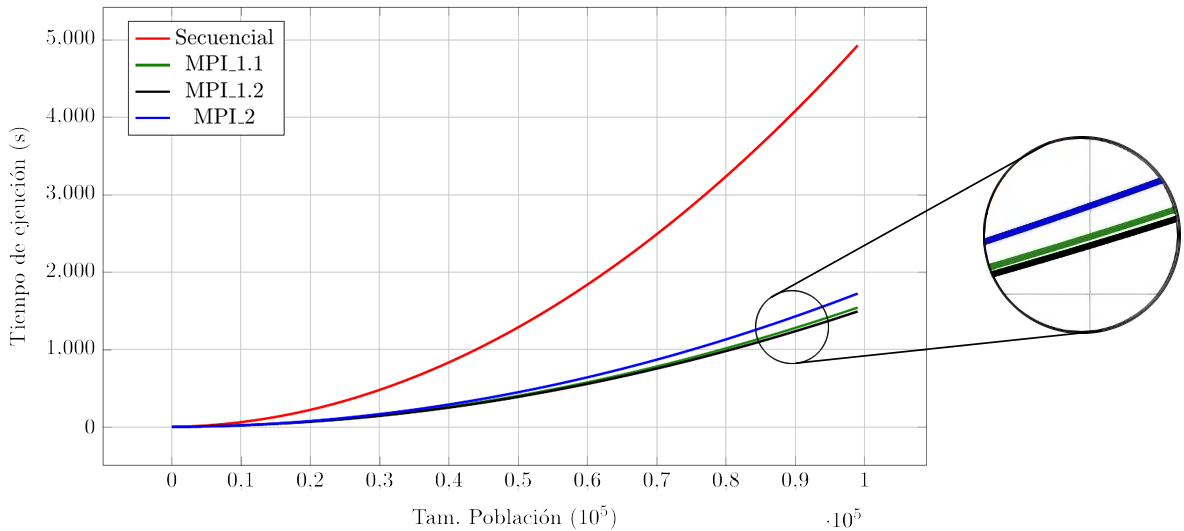
\includegraphics[width=0.8\textwidth]{images/chapter_4/knn_mpi}
				\caption{KNN - Tiempo de ejecución con las mejoras MPI}
				\label{fig:example}
			\end{figure}
			
			Las dos implementaciones son aproximadamente iguales, siendo mejor la segunda implementación de la primera mejora. Añadir los individuos categorizados de la iteración anterior cuando cada worker finaliza la búsqueda de los K vecinos más cercanos en la iteración actual, elimina el tiempo de espera que tenía la primera implementación, reduciendo levemente el tiempo.
			La segunda mejora, además de ser levemente peor en cuestión de complejidad temporal, es mucho peor en complejidad espacial. Dividir la población a predecir conlleva un mayor consumo de memoria, al tener que tener la población entera en cada proceso. En la primera mejora se reparten equitativamente los individuos nuevos, es decir, en cada iteración el master envía a un único proceso el individuo categorizado.
			
			
			\begin{enumerate}
				\item La primera mejora acaba con dos copias de la población inicial y predicha (una en el master y la otra repartida entre los procesos).
				\item La segunda mejora acaba con N copias, siendo N el número de procesos ejecutados.
			\end{enumerate}
		

			Viendo el speedup de las implementaciones, se puede concluir que al principio es mejor dividir la población a predecir, pero a largo plazo es más efectivo dividir la población categorizada, además de tener menos complejidad espacial. 
		
			\begin{figure} [!h]
				\centering
				\begin{tikzpicture}
				\begin{axis}[
					xlabel={Tam. Población ($10^4$)},
					ylabel={SpeedUp},
					xtick={0,1,2,3,4,5,6,7,8,9,10},
					legend pos=south east,			
					legend columns=3,
					grid=major,
					width=0.85\textwidth,
					height=0.35\textwidth,
					scaled x ticks=false,
					]
									
					\addplot [mark=none, color=darkgreen, line width=0.8pt] table [x index=0, y index=1, col sep=space] {files/knn_speedup.txt};
					\addplot [mark=none, color=red, line width=0.8pt] table [x index=0, y index=2, col sep=space] {files/knn_speedup.txt};
					\addplot [mark=none, color=blue, line width=0.8pt] table [x index=0, y index=3, col sep=space] {files/knn_speedup.txt};
					
									
					\addlegendentry{Ideal}
					\addlegendentry{MPI\_1}
					\addlegendentry{MPI\_2}
					
					
				\end{axis}
				\end{tikzpicture}
				\caption{KNN - SpeedUp}
			\end{figure}
			
			\newpage
		
		\subsubsection{Cluster}
		
			\begin{flushleft}
			\begin{mdframed}[roundcorner=5pt]			
				\textbf{\underline{Datos y número de procesos}}
				\vspace{0.1cm}
				
				\scriptsize	
				Este algoritmo, al contrario que KMedias, calcula la asignación de un individuo con coste lineal. Tiene coste cuadrático al procesar una población nueva. Medimos el tiempo que tarda en categorizar una nueva población de 100.000 individuos con dos variables de entrada, guardando el tiempo que tarda cada mil individuos. Ejecutando 10, 20, 35, 50, 75, 100 y 128 procesos para ver si es óptimo usar muchos procesos o genera mucha sobrecarga.
			\end{mdframed}
			\end{flushleft}	

			% TODO KNN SIN ACTUALIZAR?
			
			\begin{figure}[!h]
				\centering
				\begin{tikzpicture}
				\begin{axis}[
					xlabel={Tam. Población ($10^4$)},
					ylabel={Tiempo de ejecución (s)},
					legend style={at={(1.02,0.5)}, anchor=west},
					grid=major,
					width=\textwidth,
					height=0.45\textwidth,
					scaled x ticks=false,
					legend cell align={left},
					extra description/.code={
						\node at (1.01, 0.85) [anchor=west] {\textbf{Cores}};
					}
					]
					
					\addplot [mark=, color=red, line width=1.2pt] table [x index=0, y index=1, col sep=space] {files/cluster/knn.txt};
					\addplot [mark=, color=magenta, line width=1.2pt] table [x index=0, y index=2, col sep=space] {files/cluster/knn.txt};
					\addplot [mark=, color=blue, line width=1.2pt] table [x index=0, y index=3, col sep=space] {files/cluster/knn.txt};
					\addplot [mark=, color=orange, line width=1.2pt] table [x index=0, y index=4, col sep=space] {files/cluster/knn.txt};
					\addplot [mark=, color=black, line width=1.2pt] table [x index=0, y index=5, col sep=space] {files/cluster/knn.txt};
					\addplot [mark=, color=cyan, line width=1.2pt] table [x index=0, y index=6, col sep=space] {files/cluster/knn.txt};
					\addplot [mark=, color=darkgreen, line width=1.2pt] table [x index=0, y index=7, col sep=space] {files/cluster/knn.txt};
					
			 		
					 
					\addlegendentry{10}
					\addlegendentry{20}
					\addlegendentry{35}
					\addlegendentry{50}
					\addlegendentry{75}
					\addlegendentry{100}
					\addlegendentry{128}
					
				\end{axis}
				\end{tikzpicture}
				\caption{KNN - Pruebas en el cluster}
			\end{figure} 
			
			
			
		
			
			Los tiempos de ejecución que muestra la gráfica, marca ciertos puntos de optimalidad para distintos números de procesos ejecutados. El incremento en el número de procesos no resulta en mejoras significativas, añadiendo sobrecarga apartir de 35 procesos ejecutados, pues es similar a la ejecución con 20 procesos.
			
			
			
			
			
			
			\newpage


% ------------------------------------------------------------------------------------------------
% --- RL -----------------------------------------------------------------------------------------
% ------------------------------------------------------------------------------------------------

\section{RL}	
	
		
		
	\begin{flushleft}
	\begin{mdframed}[roundcorner=5pt]		
		\textbf{\underline{Pruebas}}
		\vspace{0.1cm}
		
		\scriptsize	
		Estas pruebas se realizan con tres distintos laberintos, ejecutando varias veces para hacer un cálculo más eficaz del tiempo de ejecución para cada laberinto. Las matrices son cuadradas, y se generan de manera aleatoria con \textit{30, 50 y 100 filas.}
	\end{mdframed}
	\end{flushleft}	
		
		
		
	\subsubsection{Algoritmo sin mejoras}

		\begin{figure}[!h]
			\centering
			\begin{tikzpicture}
			\begin{axis}[
				xlabel={Tam. del Laberinto},
				ylabel={Tiempo de ejeución (s)},
				legend pos=north west,
				grid=major,
				width=\textwidth,
				height=0.35\textwidth
				]
				
				
				\addplot [mark=none, color=red, line width=1.2pt] table [x index=0, y index=1, col sep=space] {files/rl.txt};
				\addplot [mark=none, color=darkgreen, line width=1.2pt] table [x index=0, y index=2, col sep=space] {files/rl.txt};
				
				
				\addlegendentry{Normal}
				\addlegendentry{Preprocesado}
				
				
			\end{axis}
			\end{tikzpicture}
			\caption{Tiempo de ejecución para RL}
		\end{figure}
		
		Una vez implementada este preprocesado y comparándolo con el sin procesar, los resultados son parecidos. Pero con en la búsqueda de los mejores hiper parámetros, da mejores resultados al preprocesar. No hace acciones innecesarias y le permite explorar mejor el entorno y no entrar en bucles.
		
	\subsubsection{Búsqueda de los mejores hiperparámetros}


		Para realizar la búsqueda mencionada se aplica la mejora de dividir el trabajo entre varios procesos. El master se encarga de mandar combinaciones a los workers. Dependiendo de la precisión, puede llegar a haber muchas por el poder de la combinatoria, y este proceso ser muy lento. El speedup es proporcional al número de nodos ejecutando combinaciones en paralelo.
		
		Esta búsqueda es muy útil para encontrar configuraciones que funcionen en el entorno.
		La mejora de matriz dividida no funciona correctamente, se queda en bucles en la mayoría de configuraciones que funcionan para la implementación secuencial del algoritmo. Con unos valores-Q previamente entrenados si funciona, pero la etapa de entrenamiento no funciona.

		
	
	\subsubsection{Mejora: Dividir el entorno entre los procesos}
	
		\begin{flushleft}
		\begin{mdframed}[roundcorner=5pt]		
			\textbf{\underline{Procesos}}
			\vspace{0.1cm}
			
			\scriptsize	
			Esta mejora se basa en el modelo \textit{Master-Worker}. El proceso Master divide el entorno entre todos los procesos (incluyéndose). También se encarga del punto de partida del agente (parte superior izquierda) y genera nuevos agentes conforme salen de su perímetro. Los demás procesos esperan a recibir un agente de algún proceso para poder explorar su entorno.
		\end{mdframed}
		\end{flushleft}	
		
		Esta mejora no da buenos resultados. No hemos encontrado una configuración de hiperparámetros para que el agente aprenda a llegar al destino, se queda dando vueltas en cualquier proceso. Si en vez de inicializar las experiencias a 0, usamos el mapa aprendido usando el algoritmo sin mejoras, si llega al destino. Hay una probabilidad de que el problema sea de la comunicación entre los procesos, sino de encontrar unos buenos hiperparámetros para que llegue al destino.
		
	
	\subsubsection{Mejora: Ejecuciones en paralelo}
		\begin{flushleft}
		\begin{mdframed}[roundcorner=5pt]		
			\textbf{\underline{Procesos}}
			\vspace{0.1cm}
			
			\scriptsize	
			Usando el modelo \textit{Master-Worker}. El proceso Master envia las posiciones aleatorias y el laberinto a los Workers, para que estos investiguen el laberinto y devuelven las experiencias obtenidas para que el Master haga la media y aprenda las mejores acciones para cada estado del entorno.
		\end{mdframed}
		\end{flushleft}	
		
		Esta mejora aplica la misma idea que la búsqueda de hiperparámetros, pero esta vez para investigar por completo el laberinto, desde distintos puntos de partida, para encontrar más rápidamente el mejor camino para llegar a la meta. Al ejecutar N Workers, el Master recibe la experiencia de estos procesos, provocando una reducción en el tiempo de ejecución proporcional al número de procesos ejecutados.	
		
		
		\newpage
		
	\subsubsection{Cluster}
	
			
		
		% TODO RL CLUSTER
		\color{blue}
		TODO CLUSTER, ejecutado el 27 de junio.
		\color{black}
		\newpage


% ------------------------------------------------------------------------------------------------
% --- PEV ----------------------------------------------------------------------------------------
% ------------------------------------------------------------------------------------------------	
\section{PEV}

	\begin{flushleft}			
	\begin{mdframed}[roundcorner=5pt]
		\textbf{\underline{Pruebas}}
		\vspace{0.1cm}
		
		\scriptsize		
		Para el algoritmo se ha aplicado un elitismo de 5\% conservando los mejores individuos de cada generación. Para el problema de árboles se aplica un método de control de bloating, para intentar reducir la altura de los individuos. 		
		Para mejorar la aptitud de los individuos se aplica un desplazamiento, cuya finalidad es que todos los individuos tengan valores positivos. Además de aplicar un escalado lineal, controlando la diversidad de las aptitudes.\\
		
		El método de evaluación depende del tipo de individuo. \\
		- Si es binario se calcula su valor real y se aplica una función matemática.  \\
		- Si es real, el problema del aeropuerto. \\
		- Si es árbol, el problema del cortacésped.\\
		
		Las pruebas realizadas para todas las gráficas se han ejecutado con las siguientes características:
		\begin{tcolorbox}[boxrule=0.5pt, fontupper=\small]
			\scriptsize
			Tam. Población = 100\\
			Núm. Generaciones = \{25,50,100,250,500,1000,2000\} \textbf{(Eje X)}\\
			Met. Selección: Torneo Determinístico, con un valor k=5.\\
			
			- Individuo Binario:\\
			Met. Cruce (p=0.6): Básica\\
			Met. Mutación (p=0.05): Básica \\
			P(x)=precision: \{P2: 30 bits, P10: 76 bits\}\\
			
			- Individuo Real:\\
			Met. Cruce (p=0.6): PMX\\
			Met. Mutación (p=0.3): Inserción \\
			AER(x)=aeropuerto: \{AER1: 10 vuelos, 3 pistas, AER1: 25 vuelos, 5 pistas, AER3: 100 vuelos, 10 pistas\}\\
			
			- Individuo Binario:\\
			Met. Cruce (p=0.6): Intercambio\\
			Met. Mutación (p=0.3): Terminal \\
			M(x)X(y)=matriz: \{M8X8: 8 filas, 8 columnas y 100 ticks; M100X100: 100 filas, 100 columnas y 10000 ticks\}				
			
		\end{tcolorbox}
		
	\end{mdframed}
	\end{flushleft}

	Con las tres mejoras implementadas hay que tener en cuenta el tipo de individuo para cada problema, pues dependiendo del tipo, tardará más tiempo en determinadas funciones. Además de tener en cuenta el coste de la comunicación entre procesos.
	
	Tiempo de ejecución (en segundos) de los métodos, para una operación. Es decir, el tiempo que tarda en inicializar, evaluar, seleccionar y mutar un único individuo, o cruzar dos individuos. 
	
	\vspace{0.3cm}

	Para la siguiente tabla, se marca en rojo los métodos más tardíos para cada problema. 
	\begin{itemize}
		\item Con individuos binarios, conviene dar más recursos a las operaciones de cruce y mutación.
		\item Los otros dos individuos (reales y árboles) es mejor paralelizar la función de evaluación, dependiendo de los datos de entrada de dichos problemas.
	\end{itemize}
 
	

	
	\begin{table}[!h]
		\centering
		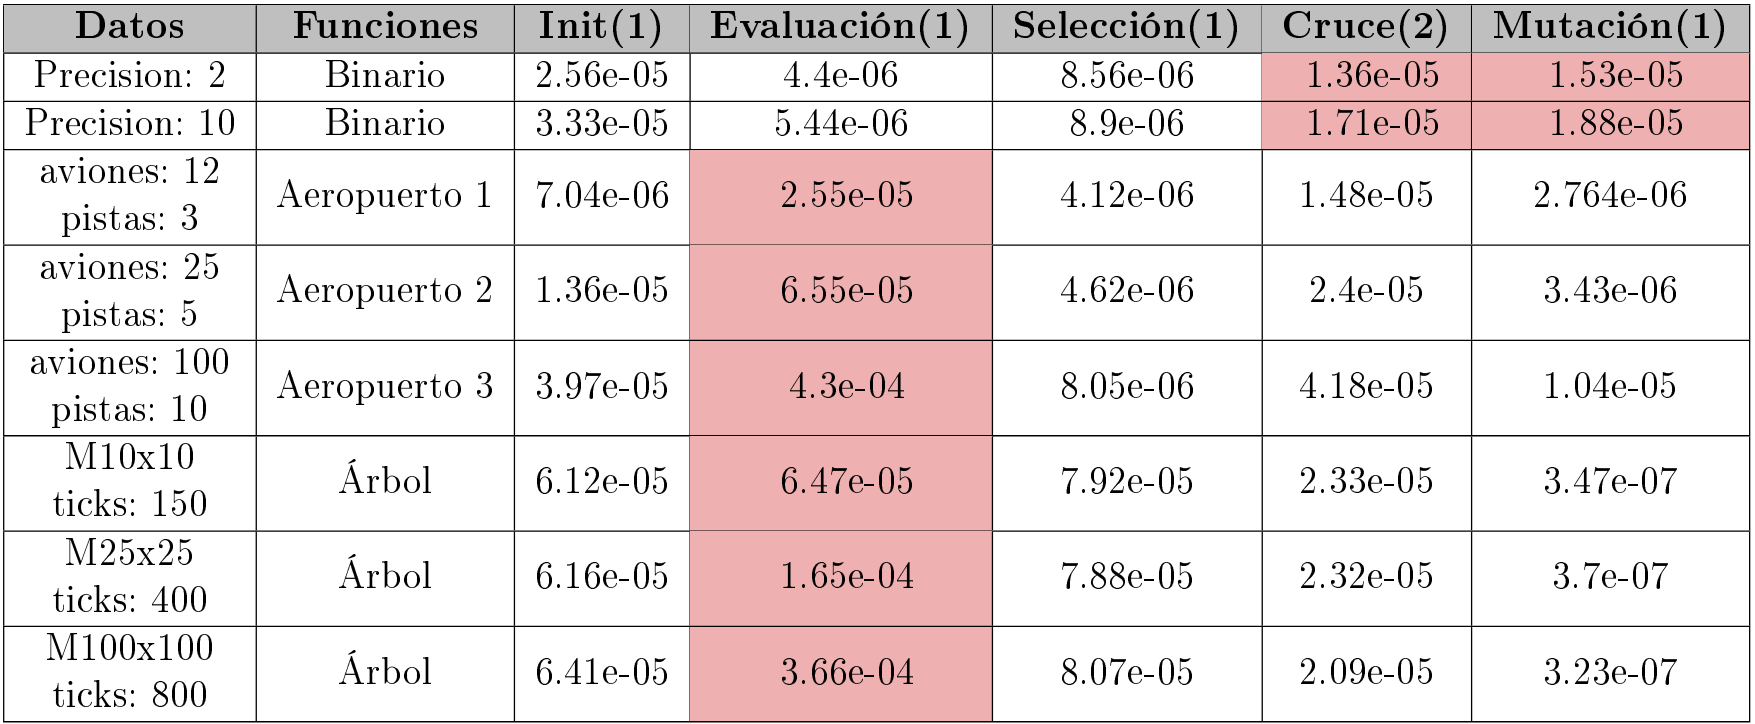
\includegraphics[width=1\textwidth]{images/chapter_4/tabla_pev}		
		\caption{PEV - Tiempos de cada método}
		\label{tab:pev}
	\end{table}
	
	%\begin{table}[!h]
	%	\centering
	%	\begin{tabular}{|c|c|c|c|c|c|c|}
	%		\hline
	%		\rowcolor{lightgray}
	%		\textbf{Datos} & \textbf{Funciones} & \textbf{Init(1)} & \textbf{Evaluación(1)} & \textbf{Selección(1)} & \textbf{Cruce(2)} & \textbf{Mutación(1)} \\
	%		\hline
	%		Precision: 2 & Binario & 2.56e-05 & 4.4e-06 & 8.56e-06 & \cellcolor{redcell} 1.36e-05 & \cellcolor{redcell} 1.53e-05 \\
	%		\hline
	%		Precision: 10 & Binario & 3.33e-05 & 5.44e-06 & 8.9e-06 & \cellcolor{redcell} 1.71e-05 & \cellcolor{redcell} 1.88e-05 \\
	%		\hline
	%		\makecell{aviones: 12 \\ pistas: 3} & Aeropuerto 1 & 7.04e-06 & \cellcolor{redcell} 2.55e-05 & 4.12e-06 & 1.48e-05 & 2.764e-06 \\
	%		\hline
	%		\makecell{aviones: 25 \\ pistas: 5} & Aeropuerto 2 & 1.36e-05 & \cellcolor{redcell} 6.55e-05 & 4.62e-06 & 2.4e-05 & 3.43e-06 \\
	%		\hline
	%		\makecell{aviones: 100 \\ pistas: 10} & Aeropuerto 3 & 3.97e-05 & \cellcolor{redcell} 4.3e-04 & 8.05e-06 & 4.18e-05 & 1.04e-05 \\
	%		\hline
	%		\makecell{M10x10 \\ ticks: 150} & Árbol & 6.12e-05 & \cellcolor{redcell} 6.47e-05 & 7.92e-05 & 2.33e-05 & 3.47e-07 \\
	%		\hline
	%		\makecell{M25x25 \\ ticks: 400} & Árbol & 6.16e-05 & \cellcolor{redcell} 1.65e-04 & 7.88e-05 & 2.32e-05 & 3.7e-07 \\
	%		\hline
	%		\makecell{M100x100 \\ ticks: 800} & Árbol & 6.41e-05 & \cellcolor{redcell} 3.66e-04 & 8.07e-05 & 2.09e-05 & 3.23e-07 \\
	%		\hline
	%	\end{tabular}
	%	\caption{PEV - Tiempos de cada método}
	%	\label{tab:pev}
	%\end{table}
	

	\subsubsection{Algoritmos sin mejoras}
	
		\begin{figure}[h!]
		\centering
		\begin{tikzpicture}
			\begin{groupplot}[
				group style={
					group size=3 by 1,
					horizontal sep=0.78cm,
					vertical sep=0.5cm},
				width=0.40\textwidth,
				height=0.40\textwidth,
				tick label style={font=\tiny} 
				]
				
				% 1
				\nextgroupplot[
				title={},
				ylabel= Tiempo de ejecución (s),
				legend style={at={(0.5,1.05)},anchor=south,legend columns=-1},
				xtick={25, 500, 1000, 1500, 2000} 
				]
				\addplot [mark=none, color=blue] table [x index=0, y index=1, col sep=space] {files/pev.txt};
				\addplot [mark=none, color=red] table [x index=0, y index=2, col sep=space] {files/pev.txt};
				\addlegendentry{\tiny P2}
				\addlegendentry{\tiny P10}
				
				% 2
				\nextgroupplot[
				title={},
				xlabel=Num. Generaciones,
				legend style={at={(0.5,1.05)},anchor=south,legend columns=-1},
				xtick={25, 500, 1000, 1500, 2000} 
				]
				\addplot [mark=none, color=blue] table [x index=0, y index=3, col sep=space] {files/pev.txt};
				\addplot [mark=none, color=green] table [x index=0, y index=4, col sep=space] {files/pev.txt};
				\addplot [mark=none, color=red] table [x index=0, y index=5, col sep=space] {files/pev.txt};
				\addlegendentry{\tiny AER 1}
				\addlegendentry{\tiny AER 2}
				\addlegendentry{\tiny AER 3}
				
				% 3
				\nextgroupplot[
				title={},
				legend style={at={(0.5,1.05)},anchor=south,legend columns=-1},
				xtick={25, 500, 1000, 1500, 2000} 
				]
				\addplot [mark=none, color=blue] table [x index=0, y index=6, col sep=space] {files/pev.txt};
				\addplot [mark=none, color=red] table [x index=0, y index=7, col sep=space] {files/pev.txt};
				\addlegendentry{\tiny M8X8}
				\addlegendentry{\tiny M100X10}
				
			\end{groupplot}        
		\end{tikzpicture}
		\caption{PEV Secuencial}
		\end{figure}

		% TODO PEV DESARROLLAR
		Como solo varía el número de generaciones, las gráficas son lineales. Si se modifica de la misma forma el tamaño de la población, serían exponenciales, y tardarían mucho tiempo para ejecutarse.
		
		\begin{enumerate}
			\item El problema que aplica individuos binarios es bastante rápido, es el que menos tiempo de ejecución tiene entre los tres problemas implementados. La complejidad de la función de evaluación es lineal O(M) siendo M el tamaño del individuo. Recorre todos los bits para convertirlo a un número real y luego ejecuta una función matemática.
			\item Para los individuos reales aumenta en relación al tamaño del problema. La complejidad de la función de evaluación es cuadrática O(N*M), siendo N el número de aviones y M las pistas. Para cada individuo recorre las pistas disponibles asignando la que menor tiempo de retraso genere al vuelo
			\item El problema de los árboles depende del número de ticks. La complejidad de la función de evaluación es lineal O(Ticks).
		\end{enumerate}
		
	\subsubsection{Mejora 2: Modelo de islas}
		

		El modelo de islas, depende de la configuración elegida. Si es el básico, se divide la población entre los workers por lo que se consigue un speedup proporcional a los procesos ejecutados. Para garantizar que funcione igual o mejor que la implementación secuencial, hay que tener una comunicación para garantizar la supervivencia de los más aptos en la población general y de vez en cuando reiniciar las poblaciones de cada proceso con los mejores resultados obtenidos. El maestro se encarga de agrupar los mejores y enviarlos a la hora del reinicio. 
		
		Si usamos la configuración en estrella o anillo, podemos ir mezclando poblaciones y tener más diversidad, siendo más probable obtener mejores resultados.

		\begin{flushleft}			
		\begin{mdframed}[roundcorner=5pt]
			\textbf{\underline{Procesos}}
			\vspace{0.1cm}
			
			\scriptsize		
			Esta prueba se realiza con \textbf{cuatro procesos}, tienen las mismas variables iniciales. Cada proceso inicializa aleatoriamente la población que va a evolucionar conforme avanzan las generaciones. Se conectan cada X (X=100) generaciones para reiniciar las poblaciones.
		\end{mdframed}
		\end{flushleft}
		
		\newpage
		
		\begin{figure}[h!]
			\centering
			\begin{tikzpicture}
			\begin{groupplot}[group style={
					group size=3 by 1,
					horizontal sep=0.78cm, 
					vertical sep=0.5cm},
				width=0.40\textwidth, height=0.22\textheight, 	
				tick label style={font=\tiny} 	
				]
				
				% 1
				\nextgroupplot[title={}, ylabel= Tiempo de ejecución (s),
				legend style={at={(0.5,1.05)},anchor=south,legend columns=2},
				xtick={25, 500, 1000, 1500, 2000}]
				\addplot [mark=none, color=blue] table [x index=0, y index=1, col sep=space] {files/pev_2mpi.txt};
				\addplot [mark=none, color=red] table [x index=0, y index=2, col sep=space] {files/pev_2mpi.txt};
				\addplot [mark=none, color=black] table [x index=0, y index=3, col sep=space] {files/pev_2mpi.txt};
				\addplot [mark=none, color=darkgreen] table [x index=0, y index=4, col sep=space] {files/pev_2mpi.txt};
				\addlegendentry{\tiny P2}
				\addlegendentry{\tiny P10}
				\addlegendentry{\tiny P2\_MPI}
				\addlegendentry{\tiny P10\_MPI}
				
				% 2
				\nextgroupplot[title={}, xlabel=Num. Generaciones,
				legend style={at={(0.5,1.05)},anchor=south,legend columns=2},
				xtick={25, 500, 1000, 1500, 2000}]
				\addplot [mark=none, color=blue] table [x index=0, y index=5, col sep=space] {files/pev_2mpi.txt};			
				\addplot [mark=none, color=red] table [x index=0, y index=7, col sep=space] {files/pev_2mpi.txt};
				\addplot [mark=none, color=black] table [x index=0, y index=6, col sep=space] {files/pev_2mpi.txt};
				\addplot [mark=none, color=darkgreen] table [x index=0, y index=8, col sep=space] {files/pev_2mpi.txt};
				\addlegendentry{\tiny AER 1}
				\addlegendentry{\tiny AER 2}
				\addlegendentry{\tiny AER 1\_MPI}
				\addlegendentry{\tiny AER 2\_MPI}
				
				
				% 3
				\nextgroupplot[title={},
				legend style={at={(0.5,1.05)},anchor=south,legend columns=-1},
				xtick={25, 500, 1000, 1500, 2000}]
				\addplot [mark=none, color=red] table [x index=0, y index=9, col sep=space] {files/pev_2mpi.txt};
				\addplot [mark=none, color=black] table [x index=0, y index=10, col sep=space] {files/pev_2mpi.txt};
				\addlegendentry{\tiny AER 3}
				\addlegendentry{\tiny AER 3\_MPI}
				
			\end{groupplot}		
			\end{tikzpicture}
			\caption{MPI - Modelo de Islas}
		\end{figure}




		El problema de los árboles calcularía resultados parecidos a estos dos gráficos. Al ser lineales y ejecutar en paralelo los procesos se obtiene un speedup aproximado al número de procesos ejecutados. Como se puede apreciar en la siguiente gráfica:


		\begin{figure}[!h]
		\centering
		\begin{tikzpicture}
			\begin{axis}[
				xlabel={Num. Generaciones ($10^3$)},
				ylabel={SpeedUp},
				legend pos=south east,
				grid=major,
				width=0.45\textwidth,
				height=0.35\textwidth,
				scaled x ticks=false,
				ymin=0, 
				ymax=5
				]
				
				
				\addplot [mark=diamond*, color=darkgreen, line width=1.2pt] table [x index=0, y index=1, col sep=space] {files/pev_2mpi_speedup.txt};
				\addplot [mark=none, color=blue, line width=0.8pt] table [x index=0, y index=2, col sep=space] {files/pev_2mpi_speedup.txt};
				\addplot [mark=none, color=black, line width=0.8pt] table [x index=0, y index=3, col sep=space] {files/pev_2mpi_speedup.txt};
				\addplot [mark=none, color=red, line width=0.8pt] table [x index=0, y index=4, col sep=space] {files/pev_2mpi_speedup.txt};
				
				
				\addlegendentry{Ideal}
				\addlegendentry{P10}
				\addlegendentry{AER3}
				\addlegendentry{M100X100}
				
				
			\end{axis}
		\end{tikzpicture}
		\caption{SpeedUp - Modelo en Islas}
		\end{figure}
		
		

	
	\subsubsection{Mejora 1: Dividir con el master}
	
		\begin{flushleft}			
		\begin{mdframed}[roundcorner=5pt]
			\textbf{\underline{Procesos}}
			\vspace{0.1cm}
			
			\scriptsize		
			Esta vez tenemos una única población. Aplicando el modelo \textit{Master-Worker} el master se encarga de dividir el trabajo entre los workers, reduciendo el tiempo de ejecución. 
			
			Para estas pruebas se ejecutan \textbf{cuatro procesos Workers}, \textbf{cinco en total} contando el Master.
		\end{mdframed}
		\end{flushleft}
		
		En cada iteración, el Master envía a los Workers el tamaño de de sub-población con el que van a trabajar. Estos inicializan la población, la evaluan y la envían de vuelta, para que hacer la selección con todos los individuos. Envía las partes de la selección a los procesos para que estos la crucen, muten y evaluen, así iterando por el número de generaciones.

		\begin{figure}[h!]
			\centering
			\begin{tikzpicture}
				\begin{groupplot}[group style={
						group size=3 by 1,
						horizontal sep=0.78cm, 
						vertical sep=0.5cm}, 
					width=0.40\textwidth, height=0.35\textwidth, 
					tick label style={font=\tiny} 
					]
					
					% 1
					\nextgroupplot[title={}, ylabel=Tiempo de ejecución (s),
					legend style={at={(0.5,1.05)},anchor=south,legend columns=2},
					xtick={25, 500, 1000, 1500, 2000}]
					\addplot [mark=none, color=blue] table [x index=0, y index=1, col sep=space] {files/pev_1_1mpi.txt};
					\addplot [mark=none, color=red] table [x index=0, y index=2, col sep=space] {files/pev_1_1mpi.txt};
					\addplot [mark=none, color=black] table [x index=0, y index=3, col sep=space] {files/pev_1_1mpi.txt};
					\addplot [mark=none, color=darkgreen] table [x index=0, y index=4, col sep=space] {files/pev_1_1mpi.txt};
					\addlegendentry{\tiny P2}
					\addlegendentry{\tiny P10}
					\addlegendentry{\tiny P2\_MPI}
					\addlegendentry{\tiny P10\_MPI}
					
					% 2
					\nextgroupplot[title={}, xlabel=Num. Generaciones,
					legend style={at={(0.5,1.05)},anchor=south,legend columns=2},
					xtick={25, 500, 1000, 1500, 2000}]
					\addplot [mark=none, color=blue] table [x index=0, y index=5, col sep=space] {files/pev_1_1mpi.txt};	
					\addplot [mark=none, color=red] table [x index=0, y index=7, col sep=space] {files/pev_1_1mpi.txt};
					\addplot [mark=none, color=black] table [x index=0, y index=6, col sep=space] {files/pev_1_1mpi.txt};
					\addplot [mark=none, color=darkgreen] table [x index=0, y index=8, col sep=space] {files/pev_1_1mpi.txt};
					\addlegendentry{\tiny AER 1}
					\addlegendentry{\tiny AER 2}
					\addlegendentry{\tiny AER 1\_MPI}
					\addlegendentry{\tiny AER 2\_MPI}
					
					% 3
					\nextgroupplot[title={},
					legend style={at={(0.5,1.05)},anchor=south,legend columns=-1},
					xtick={25, 500, 1000, 1500, 2000}]
					\addplot [mark=none, color=red] table [x index=0, y index=9, col sep=space] {files/pev_1_1mpi.txt};			
					\addplot [mark=none, color=black] table [x index=0, y index=10, col sep=space] {files/pev_1_1mpi.txt};			
					\addlegendentry{\tiny M8X8}
					\addlegendentry{\tiny MPI}
					
				\end{groupplot}	
				
			
				%\node at ($(group c1r1.south)!0.5!(group c2r1.south) + (0,-0.4cm)$) [below] {Num. Generaciones};
				
			\end{tikzpicture}
			\caption{MPI1 - Dividir Poblacion con problemas pequeños}
		\end{figure}
		
		\begin{itemize}
			\item (Gráfica izquierda). Para los problemas binarios este método no es efectivo. Se pierde mucho tiempo en el paso de mensajes. Tener para cada individuo muchos bits provoca que una población no muy grande sea inviable para aplicar esta mejora. Además de que este problema es bastante rápido.
			\item (Gráfica derecha). Aunque se controle el tamaño de los individuos, el problema es muy pequeño para alcanzar alguna mejora. Con matrices más grandes se puede mejorar.
			\item (Gráfica central). Para este tipo de problema hasta con valores pequeños se puede reducir el tiempo de ejecución. Aunque está lejos de llegar a un speedup ideal.
		\end{itemize}

		Con los problemas con pocos datos de entrada, no conviene paralelizarlos, pues son bastante rápidos. Pero al aumentar el tamaño de los problemas, puede ser beneficiosos paralelizarlos.
		
		\newpage

		\begin{figure}[!h]
			\centering
			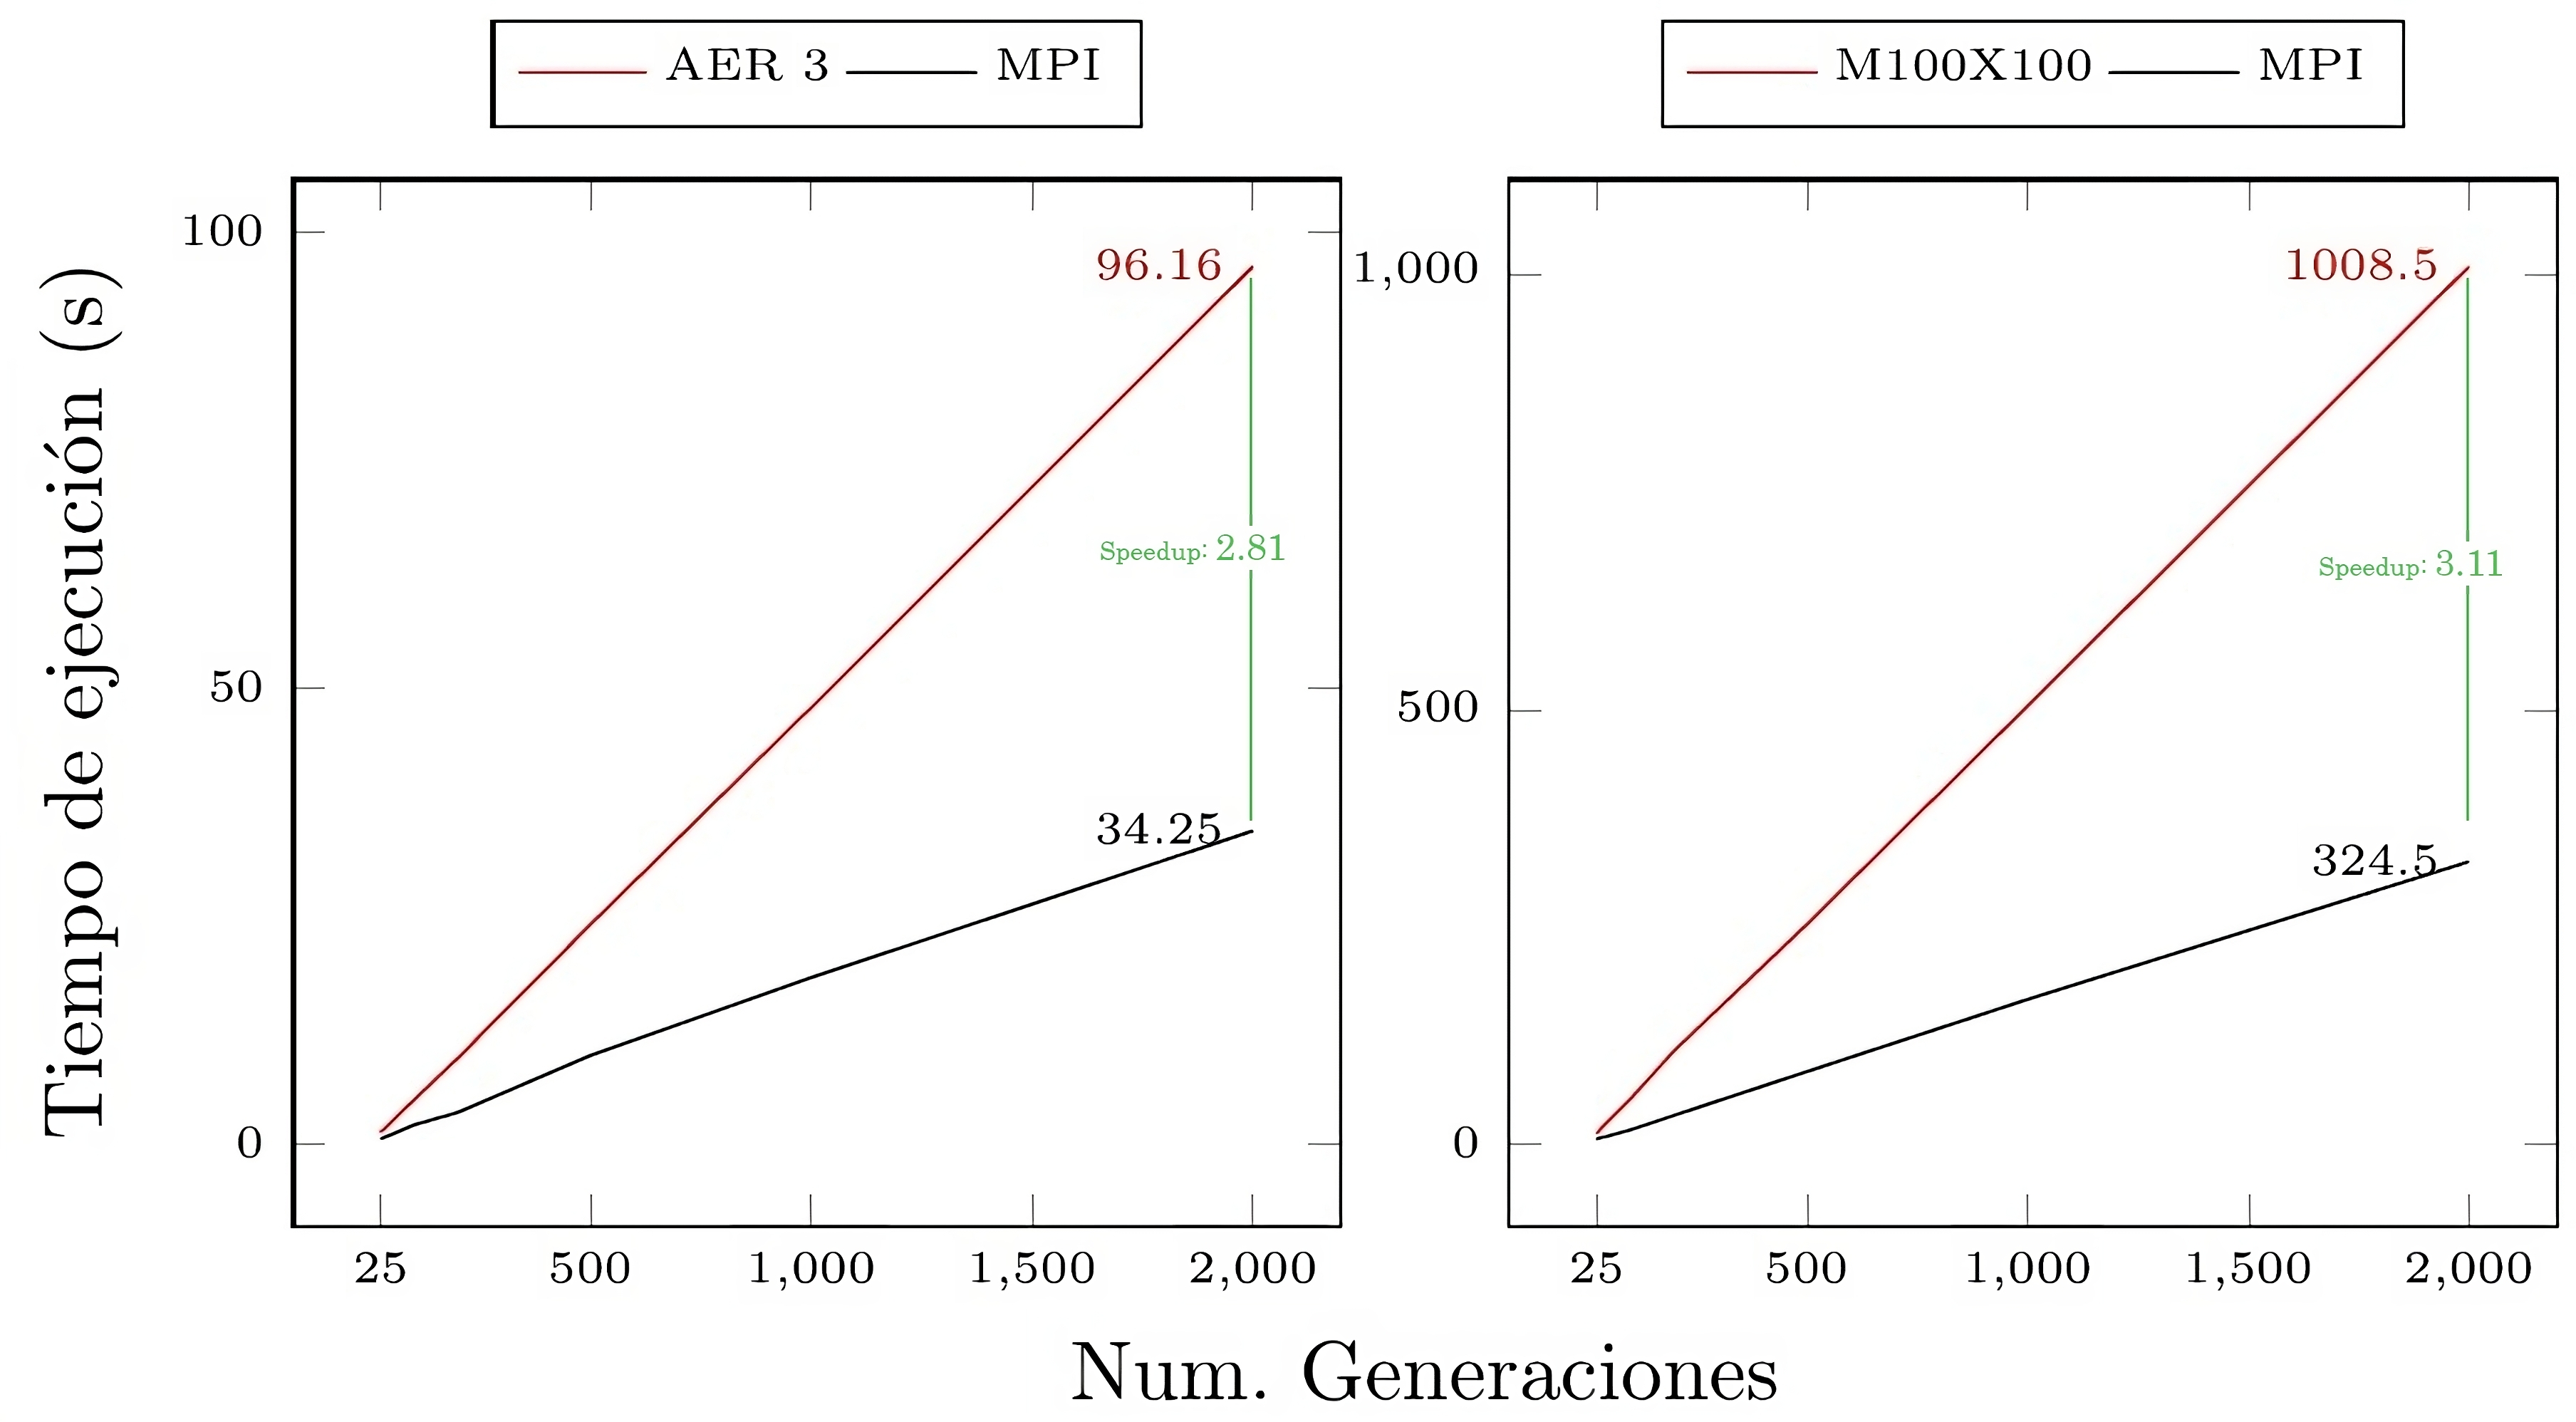
\includegraphics[width=0.7\textwidth]{images/chapter_4/pev_mpi1}
			\caption{MPI1 - Dividir Poblacion con problemas grandes}
			\label{fig:MPI1.2 - Dividir Poblacion + Speedup}
		\end{figure}

		% CODIGO DE LA IMAGEN DE ARRIBA
		%\begin{figure}[h!]
		%	\centering
		%	\begin{tikzpicture}
			%		\begin{groupplot}[group style={
					%				group size=2 by 1, % Adjust group size (2 plots horizontally)
					%				horizontal sep=0.78cm, % Adjust horizontal separation between plots
					%				vertical sep=0.5cm}, % Adjust vertical separation between plots
				%			width=0.40\textwidth, height=0.40\textwidth, % Adjust size as needed		
				%			tick label style={font=\tiny} % Adjust font size of tick labels	
				%			]
				%			
				%			% First plot
				%			\nextgroupplot[title={}, ylabel=Tiempo de ejecución (s),
				%			legend style={at={(0.5,1.05)},anchor=south,legend columns=-1},
				%			xtick={25, 500, 1000, 1500, 2000}]
				%			\addplot [mark=none, color=red] table [x index=0, y index=1, col sep=space] {files/pev_1_2mpi.txt};
				%			\addplot [mark=none, color=black] table [x index=0, y index=2, col sep=space] {files/pev_1_2mpi.txt};			
				%			\addlegendentry{\tiny AER 3}
				%			\addlegendentry{\tiny MPI}
				%			
				%			% Add value labels
				%			\node at (axis cs:2000,96.16) [text=red,left] {\tiny 96.16};
				%			\node at (axis cs:2000,34.25) [text=black,left] {\tiny 34.25};
				%			
				%			% Second plot
				%			\nextgroupplot[title={},
				%			legend style={at={(0.5,1.05)},anchor=south,legend columns=-1},
				%			xtick={25, 500, 1000, 1500, 2000}]
				%			\addplot [mark=none, color=red] table [x index=0, y index=3, col sep=space] {files/pev_1_2mpi.txt};			
				%			\addplot [mark=none, color=black] table [x index=0, y index=4, col sep=space] {files/pev_1_2mpi.txt};			
				%			\addlegendentry{\tiny M100X100}
				%			\addlegendentry{\tiny MPI}
				%			
				%			% Add value labels
				%			\node at (axis cs:2000,1008.51) [text=red,left] {\tiny 1008.5};
				%			\node at (axis cs:2000,324.52) [text=black,left]{\tiny 324.5};
				%			
				%		\end{groupplot}	
			%		
			%		% Common x-axis label
			%		\node at ($(group c1r1.south)!0.5!(group c2r1.south) + (0,-0.4cm)$) [below] {Num. Generaciones};
			%		
			%	\end{tikzpicture}
		%	\caption{MPI1.2 - Dividir Poblacion}
		%\end{figure}

		
		Como se comentó antes, al aumentar los tamaños se consiguen mejores resultados. Con estas características, la ejecución se aumenta al punto de ser buena opción aplicar esta mejora.

	\subsubsection{Mejora 3: PipeLine}
	
		\begin{flushleft}			
		\begin{mdframed}[roundcorner=5pt]
			\textbf{\underline{Procesos}}
			\vspace{0.1cm}
			
			\scriptsize		
			Mezclando el modelo \textit{Master-Worker} con segmentación, el proceso Master se encarga de generar N (número de workers) poblaciones que envía al siguiente proceso, cuando genera todos se queda en un estado de recepción de mejores individuos. Cada proceso envía su siguiente los datos procesados según su tarea, generando un flujo constante de trabajo.
		\end{mdframed}
		\end{flushleft}
		
		
		
		
		%El método de pipeline varía para cada problema. Los individuos binarios no mejoran mucho la ejecución, al tener muchos datos que enviar. 
		
		%Sin embargo los problemas con individuos reales o árboles si se pueden optimizar. La evaluación es el método que más tarda en estos dos problemas, por lo que repartir la carga de trabajo con más procesos reduce el tiempo de ejecución.
		
		\begin{figure}[!h]
			\centering
			\begin{tikzpicture}
			\begin{axis}[
				xlabel={Tam. Poblacion},
				ylabel={Tiempo (s)},
				legend pos=north west,
				grid=major,
				width=0.70\textwidth,
				height=0.4\textwidth
				]				
				
				xtick={25, 500, 1000, 1500, 2000}]
				\addplot [mark=none, color=red] table [x index=0, y index=1, col sep=space] {files/pev_3mpi.txt};
				\addplot [mark=none, color=darkgreen] table [x index=0, y index=2, col sep=space] {files/pev_3mpi.txt};
				\addplot [mark=none, color=blue] table [x index=0, y index=3, col sep=space] {files/pev_3mpi.txt};
											
				\addlegendentry{\tiny P10}
				\addlegendentry{\tiny MPI(4)}
				\addlegendentry{\tiny MPI(7)}
				
			\end{axis}
			\end{tikzpicture}
			\caption{PipeLine - Individuos Binarios}
		\end{figure}
		
		Para los individuos binarios, funciona algo mejor que la mejora anterior, con el funcionamiento de pipeline no se pierde tanto tiempo con el paso de mensajes de individuos binarios, y aunque sea poco, se puede reducir el tiempo de ejecución.
			
		Al tener varias poblaciones ejecutándose al mismo tiempo no se puede tener una población muy grande. A partir de un tamaño de 1000 individuos no se puede ejecutar con dos decimales de precisión con el ordenador de propósito general, y con 500 individuos es el máximo tamaño de población si se usan 10 decimales de precisión.
	 
	 
	\begin{flushleft}
	 	\begin{mdframed}[roundcorner=5pt]			 		
		 		\small
		 		\color{darkgreen} 1. Cuatro procesos: \color{black}
		 		\vspace{-0.3cm}
		 		\scriptsize
		 		\begin{itemize}
		 			\item Master se encarga de inicializar
		 			\vspace{-0.1cm}
		 			\item Worker1: evaluación y selección, procesos que no tardan mucho en ejecutarse.
		 			\vspace{-0.1cm}
		 			\item Worker2: cruce
		 			\vspace{-0.1cm}
		 			\item Worker3: mutación
		 		\end{itemize}
		 		\small
		 		\color{blue} 2. Siete procesos. \color{black} 	\scriptsize	Se duplica el numero de workers en cada pipe.
  
	 	\end{mdframed}
 		\end{flushleft}
		 		
	 Para los individuos reales y arboles, al no tener tantos elementos por individuo, esta mejora funciona correctamente. Estos dos individuos tienen la misma implementación al tener tiempos similares y perder la mayor parte del tiempo en la evaluación de los individuos.
	 
	 
	 \begin{figure}[!h]
		 	\centering
		 	\begin{tikzpicture}
	 		\begin{axis}[
	 			xlabel={Tam. Poblacion},
	 			ylabel={Tiempo (s)},
	 			legend pos=north west,
	 			grid=major,
	 			width=0.70\textwidth,
	 			height=0.45\textwidth
	 			]				
	 			
	 			xtick={25, 500, 1000, 1500, 2000}]
	 			\addplot [mark=none, color=red] table [x index=0, y index=4, col sep=space] {files/pev_3mpi.txt};			
	 			\addplot [mark=none, color=darkgreen] table [x index=0, y index=5, col sep=space] {files/pev_3mpi.txt};
	 			\addplot [mark=none, color=blue] table [x index=0, y index=6, col sep=space] {files/pev_3mpi.txt};	
	 			\addlegendentry{\tiny AER3}
	 			\addlegendentry{\tiny MPI(6)}
	 			\addlegendentry{\tiny MPI(10)}
	 			
	 		\end{axis}
		 	\end{tikzpicture}
		 	\caption{PipeLine - Individuos Reales}
	 \end{figure}
	 
	 

		%\begin{figure}[h!]
		%	\centering
		%	\begin{tikzpicture}
		%	\begin{groupplot}[group style={
		%			group size=3 by 1,
		%			horizontal sep=0.78cm, 
		%			vertical sep=0.5cm},
		%		width=0.40\textwidth, height=0.40\textwidth, 
		%		tick label style={font=\tiny} 
		%		]
		%		
		%		% 1
		%		\nextgroupplot[title={}, ylabel=Tiempo de ejecución (s),
		%		legend pos=north west,
		%		xtick={25, 500, 1000, 1500, 2000}]
		%		\addplot [mark=none, color=red] table [x index=0, y index=1, col sep=space] {files/pev_3mpi.txt};
		%		\addplot [mark=none, color=darkgreen] table [x index=0, y index=2, col sep=space] {files/pev_3mpi.txt};
		%		\addplot [mark=none, color=blue] table [x index=0, y index=3, col sep=space] {files/pev_3mpi.txt};							
		%		\addlegendentry{\tiny P10}
		%		\addlegendentry{\tiny MPI(4)}
		%		\addlegendentry{\tiny MPI(7)}
		%		
		%		
		%		% 2
		%		\nextgroupplot[title={},
		%		legend pos=north west,
		%		xtick={25, 500, 1000, 1500, 2000}]
		%		\addplot [mark=none, color=red] table [x index=0, y index=4, col sep=space] {files/pev_3mpi.txt};			
		%		\addplot [mark=none, color=darkgreen] table [x index=0, y index=5, col sep=space] {files/pev_3mpi.txt};
		%		\addplot [mark=none, color=blue] table [x index=0, y index=6, col sep=space] {files/pev_3mpi.txt};	
		%		\addlegendentry{\tiny AER3}
		%		\addlegendentry{\tiny MPI(6)}
		%		\addlegendentry{\tiny MPI(10)}
		%		
		%	\end{groupplot}	
		%	
		%	\node at ($(group c1r1.south)!0.5!(group c2r1.south) + (0,-0.4cm)$) [below] {Num. Generaciones};
		%	\end{tikzpicture}
		%	\caption{MPI3 - PipeLine}
		%\end{figure}

		
		
		%\begin{flushleft}
		%	\begin{mdframed}[roundcorner=5pt]
		%		\normalsize
		%		\textbf{Binarios}	
		%		
		%		\small
		%		\color{darkgreen} 1. Cuatro procesos: \color{black}
		%		\vspace{-0.3cm}
		%		\scriptsize
		%		\begin{itemize}
		%			\item Master se encarga de inicializar
		%			\vspace{-0.1cm}
		%			\item Worker1: evaluación y selección, procesos que no tardan mucho en ejecutarse.
		%			\vspace{-0.1cm}
		%			\item Worker2: cruce
		%			\vspace{-0.1cm}
		%			\item Worker3: mutación
		%		\end{itemize}
		%		\small
		%		\color{blue} 2. Siete procesos. \color{black} 	\scriptsize	Se duplica el numero de workers en cada pipe.	
		%		
		%		\vspace{0.2cm}
		%		
		%		\normalsize		
		%		\textbf{Reales} \small (Solo aumenta el número de workers en el método de evaluación.)	
		%		
		%		
		%		\normalsize		
		%		\color{darkgreen} 1. Seis procesos: \color{black}
		%		\vspace{-0.3cm}
		%		\scriptsize
		%		\begin{itemize}			
		%			\item Master se encarga de inicializar
		%			\vspace{-0.1cm}
		%			\item Worker [1, 4]: evaluación, función que más tarda			
		%			\vspace{-0.1cm}
		%			\item Worker 5:  selección, cruce y mutación						
		%			\vspace{-0.1cm}
		%		\end{itemize}
		%		\small
		%		\color{blue} 2. Diez procesos. \color{black} \scriptsize Se duplica el numero de workers en cada pipe.
		%		
		%		\vspace{0.2cm}
		%		\normalsize
		%		\textbf{Arboles:} \small Es igual que la implementación de individuos reales, pues la evaluación es el método que más tarda.			
		%	\end{mdframed}
		%\end{flushleft}


		\begin{flushleft}
		\begin{mdframed}[roundcorner=5pt]					
			\normalsize		
			\textbf{Reales} \small (Solo aumenta el número de workers en el método de evaluación.)	
			
			
			\normalsize		
			\color{darkgreen} 1. Seis procesos: \color{black}
			\vspace{-0.3cm}
			\scriptsize
			\begin{itemize}			
				\item Master se encarga de inicializar
				\vspace{-0.1cm}
				\item Worker [1, 4]: evaluación, función que más tarda			
				\vspace{-0.1cm}
				\item Worker 5:  selección, cruce y mutación						
				\vspace{-0.1cm}
			\end{itemize}
			\small
			\color{blue} 2. Diez procesos. \color{black} \scriptsize Se duplica el numero de workers en cada pipe.
			
			\vspace{0.2cm}
			\normalsize
			\textbf{Arboles:} \small Es igual que la implementación de individuos reales, pues la evaluación es el método que más tarda.			
		\end{mdframed}
		\end{flushleft}



		\begin{flushleft}
			Estos datos se calcularon teniendo en cuenta los tiempos de ejecución para cada método (Tabla \ref{tab:pev}).
		\end{flushleft}
		
		\begin{table}[!h]				
		\centering
		\begin{tabular}{|c|c|c|c|}
			\hline
			\rowcolor{lightgray}
			\textbf{Evaluación} & \textbf{Selección} & \textbf{Cruce} & \textbf{Mutación}\\
			\hline
			400e-06s  & 8e-06 & 40e-06 & 10e-06\\ 
			\hline
		\end{tabular}
		\caption{PEV - Tiempos de aproximados usados}
		\label{tab:tiempos_aprox}
		\end{table}
		
		
		Al juntar los últimos tres métodos, tarda un tiempo aproximado de 58e-06. 6.9 veces más rápido que la evaluación. Por simplicidad, es mejor ejecutar potencias de dos procesos, para hacer una división equitativa.
	
	\subsubsection{Cluster}
	
			\begin{flushleft}
			\begin{mdframed}[roundcorner=5pt]			
				\textbf{\underline{Datos y número de procesos}}
				\vspace{0.1cm}
				
				\scriptsize	
				Para la siguiente prueba se ejecuta la primera mejora, el \textit{Master} se encarga de dividir la población entre los procesos, con 10, 20, 50 y 100 procesos \textit{Workers}. Se ejecutan 25 generaciones, con las siguientes poblaciones [1000, 2000, 5000, 7000].
			\end{mdframed}
			\end{flushleft}	
			
			Ambos problemas, como mencionamos anteriormente tiene tiempos parecidos. La \textbf{sobrecarga se empieza a notar con cincuenta procesos}, pues la mejora entre usar veinte y cincuenta es de un 25\% mas rápida, además de ser más eficaz que usar cien procesos.
			
			\newpage
			
			\begin{figure}[!h]
				\centering
				\begin{tikzpicture}
				\begin{axis}[
					xlabel={Tam. Población ($10^3$)},
					ylabel={Tiempo de ejecución (s)},
					legend style={at={(1.02,0.5)}, anchor=west},
					grid=major,
					width=\textwidth,
					height=0.45\textwidth,
					scaled x ticks=false,
					legend cell align={left},
					extra description/.code={
						\node at (1.01, 0.72) [anchor=west] {\textbf{Cores}};
					}
					]
					
					\addplot [mark=*, color=red, line width=1.2pt] table [x index=0, y index=1, col sep=space] {files/cluster/pevReal.txt};
					\addplot [mark=square*, color=magenta, line width=1.2pt] table [x index=0, y index=2, col sep=space] {files/cluster/pevReal.txt};
					\addplot [mark=triangle*, color=black, line width=1.2pt] table [x index=0, y index=3, col sep=space] {files/cluster/pevReal.txt};
					\addplot [mark=star, color=darkgreen, line width=1.2pt] table [x index=0, y index=4, col sep=space] {files/cluster/pevReal.txt};
					
					
					\addlegendentry{10}
					\addlegendentry{20}
					\addlegendentry{50}
					\addlegendentry{100}
					
				\end{axis}
				\end{tikzpicture}
				\caption{PEV Real - Tiempo de ejecución en el Cluster}
			\end{figure}
			
			
			
			
		
			
			\begin{figure}[!h]
				\centering
				\begin{tikzpicture}
				\begin{axis}[
					xlabel={Tam. Población ($10^3$)},
					ylabel={Tiempo de ejecución (s)},
					legend style={at={(1.02,0.5)}, anchor=west},
					grid=major,
					width=\textwidth,
					height=0.45\textwidth,
					scaled x ticks=false,
					legend cell align={left},
					extra description/.code={
						\node at (1.01, 0.72) [anchor=west] {\textbf{Cores}};
					}
					]
					
					\addplot [mark=*, color=red, line width=1.2pt] table [x index=0, y index=1, col sep=space] {files/cluster/pevArbol.txt};
					\addplot [mark=square*, color=magenta, line width=1.2pt] table [x index=0, y index=2, col sep=space] {files/cluster/pevArbol.txt};
					\addplot [mark=triangle*, color=black, line width=1.2pt] table [x index=0, y index=3, col sep=space] {files/cluster/pevArbol.txt};
					\addplot [mark=star, color=darkgreen, line width=1.2pt] table [x index=0, y index=4, col sep=space] {files/cluster/pevArbol.txt};
					
					
					\addlegendentry{10}
					\addlegendentry{20}
					\addlegendentry{50}
					\addlegendentry{100}
						
					\end{axis}
				\end{tikzpicture}
				\caption{PEV Arbol - Tiempo de ejecución en el Cluster}
			\end{figure}
			
			
			\newpage
			
\section{Redes Neuronales}


		\begin{flushleft}
		\begin{mdframed}[roundcorner=5pt]	
			
			\textbf{\underline{Pruebas}}
			\vspace{0.1cm}
			
			\scriptsize	
			Se usa una población de 80 individuos, generados previamente de manera no aleatoria, para tener una concordancia con valores reales, de altura y masa corporal, y así calcular IMCs con concordancia. Se generan con combinaciones en las cuales se aumenta la altura cada vez que se crean 10 individuos con diferentes pesos. Los individuos oscilan en alturas de [150, 200]cms.										
			
		\end{mdframed}
		\end{flushleft}
		
		\subsubsection{Mejora 1: PipeLine}
		
			\begin{flushleft}			
				\begin{mdframed}[roundcorner=5pt]
					\textbf{\underline{Procesos}}
					\vspace{0.1cm}
					
					\scriptsize		
					Aplicando el modelo \textit{Master-Worker} junto con segmentación, cada proceso se encarga de un determinado numero de capas. El proceso Master se encarga de empezar a categorizar los individuos, ejecutando el metodo forward() en sus capas, una vez llega a su última capa envía los datos que ha procesado al siguiente proceso, y genera otro individuo. Los procesos procesan los individuos que reciben, generando un flujo de individuos. El último proceso se encarga de evaluar y gestionar los errores para enviar hacia atrás (método de propagación hacia atrás).
				\end{mdframed}
			\end{flushleft}
		
		
		
			\begin{tcolorbox}[boxrule=0.5pt]
				\scriptsize
				Para la siguiente prueba se utiliza una red neuronal con capa oculta de 1x5, es decir, una capa y cinco nodos.		
			\end{tcolorbox}



			\begin{figure}[!h]
				\centering
				\begin{tikzpicture}
					\begin{axis}[
						xlabel={Num. Repeticiones ($10^3$)},
						ylabel={Tiempo de ejeución (s)},
						legend pos=north west,
						grid=major,
						width=\textwidth,
						height=0.45\textwidth,
						scaled x ticks=false,
						]
						
						% Plot data from the file without markers, with different colors, and thicker lines
						\addplot [mark=none, color=red, line width=1.2pt] table [x index=0, y index=1, col sep=space] {files/redneu1.txt};
						\addplot [mark=none, color=darkgreen, line width=1.2pt] table [x index=0, y index=2, col sep=space] {files/redneu1.txt};
						\addplot [mark=none, color=black, line width=1.2pt] table [x index=0, y index=3, col sep=space] {files/redneu1.txt};
						
						% Add legends
						\addlegendentry{Secuencial}
						\addlegendentry{Síncrono}
						\addlegendentry{Asíncrono}
						
						
					\end{axis}
				\end{tikzpicture}
				\caption{MPI1 - Red Neuronal}
			\end{figure}

			Una vez implementado para una red neuronal pequeña, no reduce el tiempo de ejecución. En programación evolutiva, el flujo de mensajes es unidireccional, y no se pierde tanto tiempo entre mensajes. Este algoritmo tiene dos métodos en diferentes direcciones, provocando un \textbf{flujo bidireccional}, y la comunicación entre procesos se ralentiza. Usando mensajes \textbf{asíncronos}, permite a cada proceso ejecutar antes el cálculo de forward y cuando recibe los errores los actualiza. Reduce muy poco el tiempo comparándolo con la versión síncrona, pero empeora la predicción del modelo.
			También hay que tener en cuenta que el flujo de mensajes hace que el modelo aprenda con valores desactualizados. Y dependiendo de la población puede haber un bucle en el cual aumenta y reduce los pesos, provocando un entrenamiento erróneo.

			% TODO REDNEU 5X50
			
			\color{blue} TODO PROBAR CON 5X50
			
			\color{black}
			\newpage
			
		\subsubsection{Mejora 2: Dividir el trabajo en procesos}
		
			\begin{flushleft}			
			\begin{mdframed}[roundcorner=5pt]
				\textbf{\underline{Procesos}}
				\vspace{0.1cm}
				
				\scriptsize		
				Para esta mejora se aplica el modelo \textit{Master-Worker}. El proceso Master se encarga de dividir eficazmente la población, para el máximo rendimiento de la red neuronal. Cada Worker se encarga de entrenar con una población distinta para aprender correctamente como categorizar los individuos. Una vez se ha terminado la fase de entrenamiento, envían al Master todas sus experiencias para que este haga la media y pueda aprender a predecir correctamente. (Para el correcto funcionamiento la red neuronal tiene que ser grande, si no no se puede garantizar que prediga correctamente para todos los individuos de la población)
			\end{mdframed}
			\end{flushleft}

			Para dividir la población de entrenamiento, aplicando la idea de fine-tuning, entre los procesos hay que tener mucho cuidado. La repartición de individuos es crucial para un correcto aprendizaje de la red. Si cada proceso tiene la misma población de entrenamiento, se reduce el tiempo de ejecución en relación al número de procesos ejecutados, pero no garantiza buenas predicciones, pues la media sería parecida. A no ser que cada proceso inicialmente tuviese pesos distintos, aunque no se podría garantizar un buen entrenamiento. Sin embargo dividiendo la población de manera eficiente se podría intentar provocar que cada proceso aprendiese unos ciertos intervalos, y con una red grande ciertos nodos se especializan en unos datos, y no se entrelazan los resultados, llegando a reducir el tiempo y entrenar correctamente.
			
			\begin{figure}[!h]
				\centering
				\begin{tikzpicture}
				\begin{axis}[
					xlabel={Num. Repeticiones ($10^3$)},
					ylabel={Tiempo de ejeución (s)},
					legend pos=north west,
					grid=major,
					width=\textwidth,
					height=0.45\textwidth,
					scaled x ticks=false,
					]
					
					
					\addplot [mark=none, color=red, line width=1.2pt] table [x index=0, y index=1, col sep=space] {files/redneu2.txt};
					\addplot [mark=none, color=darkgreen, line width=1.2pt] table [x index=0, y index=2, col sep=space] {files/redneu2.txt};
					\addplot [mark=none, color=black, line width=1.2pt] table [x index=0, y index=3, col sep=space] {files/redneu2.txt};
					
					
					\addlegendentry{Secuencial}
					\addlegendentry{MPI(2)}
					\addlegendentry{MPI(4)}
					
					
				\end{axis}
				\end{tikzpicture}
				\caption{MPI2 - Red Neuronal Dividiendo entrenamiento}
			\end{figure}
			
			Esta prueba se ejecutó con 80 individuos en la población de entrenamiento, sobre una red neuronal con diez capas ocultas y diez nodos por capa (10x10). Si aumentamos o reducimos la población o la estructura de la red, el tiempo será proporcional.
			Al dividir la fase de entrenamiento se puede alcanzar un speedup aproximado al ideal, pero lo difícil es encontrar los valores concretos de los hiper parámetros y la repartición del entrenamiento para tener una buena red neuronal que cumpla con el funcionamiento deseado. Para ello se puede realizar una búsqueda en paralelo comprobando los mejores resultados, tanto variando la tasa de aprendizaje como la repartición de los individuos con los cuales se entrena al modelo.
			
			Para realizar la búsqueda de mejores hiper parámetros se ejecuta, con los mismos pesos, varias veces con diferentes valores, almacenando los mejores resultados y cuando se obtienen. Con cien repeticiones con un tamaño de población de ochenta individuos y una precisión de 0.01 se pueden comprobar los resultados en un intervalo de [0.01,0.20].


			% TODO CENTRAR BIEN
			\begin{figure}[!h]
				\centering
				
				
				\begin{subfigure}[t]{0.35\textwidth}
					\begin{tikzpicture}
					\begin{axis}[
						ybar,
						bar width=0.35cm,
						ylabel={Tiempo de ejecución (s)},
						xlabel={Capa Oculta},
						symbolic x coords={5x1, 10x2, 20x3},
						xtick=data,
						enlarge x limits=0.2,
						ymin=0,
						legend pos={north west},
						area legend
						]
						
						\addplot+[ybar, pattern=vertical lines, draw=black] plot coordinates 
						{(5x1, 2.342097799992189) (10x2, 10.170772599987686) (20x3, 45.124263799982145)};
						\addplot+[ybar, pattern=grid, draw=black] plot coordinates 
						{(5x1, 0.6505134999752045) (10x2, 2.6451210000086576) (20x3, 12.60217950004153)};
						
						
						
						\legend{Secuencial, MPI(4)}
					\end{axis}
					\end{tikzpicture}
					\label{fig:redneubusqueda}
					\caption{Grafica + SpeedUp}
				\end{subfigure}
				\hfill
				\begin{subfigure}[t]{0.55\textwidth}
					\centering
					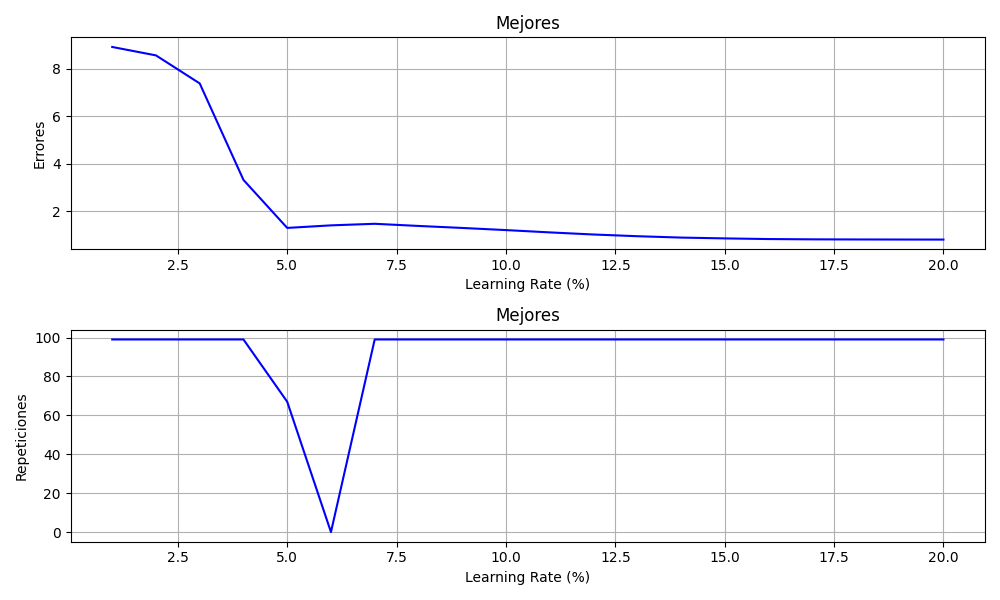
\includegraphics[width=0.8\textwidth,height=0.8\textwidth]{images/chapter_4/redneu_err}
					
					\caption{MPI - MergeSort}
					\label{fig:Errores}
				\end{subfigure}
				
				\caption{Mejoras MPI de las ordenaciones}
				\label{fig:Red Neuronal - Busqueda}
			\end{figure}




			Se ejecuta el algoritmo sobre varias configuraciones, en cada configuración siempre se utilizan los mismos pesos, para así comprobar cuales son los mejores hiper parámetros.
			
			A la derecha se pueden ver los gráficos de la evolución, siendo el de arriba los errores cometidos en cada tasa de aprendizaje, y el de abajo cuando se obtienen menos errores.